%% Copernicus Publications Manuscript Preparation Template for LaTeX Submissions
%% Please use the following documentclass and journal abbreviations for preprints and final revised papers.
%% 2-column papers and preprints
\documentclass[gmd, manuscript]{copernicus}
%% \usepackage commands included in the copernicus.cls:
%\usepackage[german, english]{babel}
%\usepackage{tabularx}
%\usepackage{cancel}
%\usepackage{multirow}
%\usepackage{supertabular}
%\usepackage{algorithmic}
%\usepackage{algorithm}
%\usepackage{amsthm}
%\usepackage{float}
%\usepackage{subfig}
%\usepackage{rotating}
\usepackage{enumitem}

\usepackage[colorinlistoftodos,textwidth=0.4in,textsize=tiny]{todonotes}

\begin{document}

\title{Applications of Machine Learning and Artificial Intelligence in Tropospheric Ozone Research}

\Author[1,*]{Sebastian H. M.}{Hickman}
\Author[2,*]{Makoto M.}{Kelp}
\Author[3,a*]{Paul T.}{Griffiths}
\Author[4,*]{Kelsey}{Doerksen}
\Author[5,*]{Kazuyuki}{Miyazaki}
\Author[5,*]{Elyse A.}{Pennington}
\Author[6,*]{Gerbrand}{Koren}
\Author[7,*]{Fernando}{Iglesias-Suarez}
\Author[8,16*]{Martin G.}{Schultz}
\Author[9,10]{Kai-Lan}{Chang}
\Author[9]{Owen R.}{Cooper}
\Author[3]{Alex}{Archibald}
\Author[11,12]{Roberto}{Sommariva}
\Author[13]{David}{Carlson}
\Author[14]{Hantao}{Wang}
\Author[14]{J. Jason}{West}
\Author[15]{Zhenze}{Liu}


\affil[1]{Yusuf Hamied Department of Chemistry, University of Cambridge, Cambridge, UK}
\affil[2]{Doerr School of Sustainability, Stanford University, CA, USA}
\affil[3]{National Centre for Atmospheric Science, Cambridge University}
\affil[4]{Department of Computer Science, University of Oxford}
\affil[5]{Jet Propulsion Laboratory, California Institute of Technology, Pasadena, CA, USA}
\affil[6]{Copernicus Institute of Sustainable Development, Utrecht University, Utrecht, the Netherlands}
\affil[7]{Predictia Intelligent Data Solutions S.L., Santander, Spain}
\affil[8]{J\"ulich Supercomputing Centre, Forschungszentrum J\"ulich, J\"ulich, Germany}
\affil[9]{NOAA Chemical Sciences Laboratory, Boulder, CO, USA}
\affil[10]{Cooperative Institute for Research in Environmental Sciences, University of Colorado Boulder,}
\affil[11]{ School of Geography, Earth and Environmental Sciences, University
of Birmingham, Birmingham, UK}
\affil[12]{School of Chemistry, University of Leicester, Leicester, UK}
\affil[13]{Civil and Environmental Engineering, Duke University, NC, USA}
\affil[14]{Department of Environmental Sciences and Engineering, University of North Carolina, Chapel Hill, NC, USA}
\affil[15]{Jiangsu Key Laboratory of Atmospheric Environment Monitoring and Pollution Control, School of Environmental Science and Engineering, Nanjing University of Information Science and Technology, Nanjing, China}
\affil[16]{Department of Mathematics and Computer Science, University of Cologne, Cologne, Germany}
\affil[a]{now at: School of Chemistry, Bristol University, UK.}
\affil[*]{These authors contributed equally to this work.}

\correspondence{Paul Griffiths (paul.griffiths@ncas.ac.uk)}

\runningtitle{TOAR-ML4O3}
\runningauthor{Hickman, Kelp, Griffiths \emph{et al.}}
\firstpage{1}

\maketitle

\begin{abstract}

Machine learning (ML) is transforming atmospheric chemistry, offering powerful tools to address challenges in tropospheric ozone research, a critical area for climate resilience and public health. As in adjacent fields, ML approaches complement existing research by learning patterns from ever-increasing volumes of atmospheric and environmental data relevant to ozone. We highlight the rapid progress made in the field since Phase 1 of the Tropospheric Ozone Assessment Report (TOAR), focussing particularly on the most active areas of research, namely short-term ozone forecasting, emulation of atmospheric chemistry and the use of remote sensing for ozone estimation. Despite these advances, many challenges in the field remain, including those generally found in applying ML to the physical sciences, 
% including the quality of data, benchmarks, and limited model generalization and explainability, 
and further challenges particular to ozone modeling. This review provides a comprehensive synthesis of recent advancements, highlights critical challenges, and proposes actionable pathways to further advance ML applications in ozone research. Achieving this potential will require close collaborations across atmospheric chemistry, ML and computational science, aimed at addressing key challenges such as the development of global benchmark datasets and robust, explainable models.

\end{abstract}

\introduction  %% \introduction[modified heading if necessary]

The ML4O3 working group was established as part of the second phase of the IGAC Tropospheric Ozone Assessment Report (TOAR). The group focuses on the application of machine learning (ML) concepts and methods, promoting dialogue between researchers in machine learning and tropospheric ozone communities. The motivation of this group is to allow the atmospheric chemistry community to capitalize on the potential of ML and AI techniques that has recently been demonstrated for weather and climate applications. The ML tasks that were addressed by the group included identifying complex patterns, interpolating missing values, detecting errors or anomalies, and identifying air pollution regimes. The working group aimed to contribute to both fundamental scientific understanding of the processes controlling ozone, and to improved air quality monitoring and forecasting.


Tropospheric ozone is a harmful atmospheric pollutant and an important greenhouse gas, contributing to both environmental and public health issues. Long-term exposure to elevated ozone levels is linked to hundreds of thousands of premature deaths globally each year \citep{malashock_global_2022, malley_updated_2017, health_effects_institute_state_2024}. Short-term exposure can cause serious negative health impacts \citep{bell_who_2014} including reduced lung function, particularly in individuals with pre-existing medical conditions \citep{us2020integrated}. Beyond its health impacts, tropospheric ozone significantly damages vegetation in natural ecosystems and agricultural fields \citep{mills_ozone_2018} and can act as a climate forcer in the upper troposphere. In addition, ozone plays a critical role in tropospheric chemistry, both as a source of oxidants and as a primary oxidant itself \citep{monks_tropospheric_2015}.

Ozone is challenging to simulate accurately \citep{young_tropospheric_2018}, also for ML models, because it is not directly emitted into the troposphere but is photochemically produced in the presence of sunlight by reactions involving its precursor gases: carbon monoxide (CO), methane (CH$_4$), volatile organic compounds (VOCs), and nitrogen oxides (NO$_X$, NO+NO$_2$). In addition, ozone is transported from the stratosphere into the troposphere. The removal of tropospheric ozone is controlled by chemical loss and deposition to the surface \citep{archibald_tropospheric_2020}. The lifetime of ozone in the troposphere ranges from days to weeks, depending on local chemical and meteorological conditions \citep{lelieveld_what_2000, monks_tropospheric_2015}. This variability allows ozone and its precursors to be transported over long distances from their sources \citep{fiore_multimodel_2009}.

The complex coupling of these chemical and physical processes control the local concentrations of ozone across different spatial and temporal scales, as detailed in Figure \ref{fig:difficulties1}. Traditionally, concentrations of ozone and other chemical species are calculated using numerical models of the atmosphere that represent these processes across a wide range of spatial scales, from high-resolution urban models (meter-scale) to global chemistry-climate models with resolutions ranging from tens to hundreds of kilometers (e.g. \citet{Morgenstern2017}). 


\begin{figure}
    \centering
    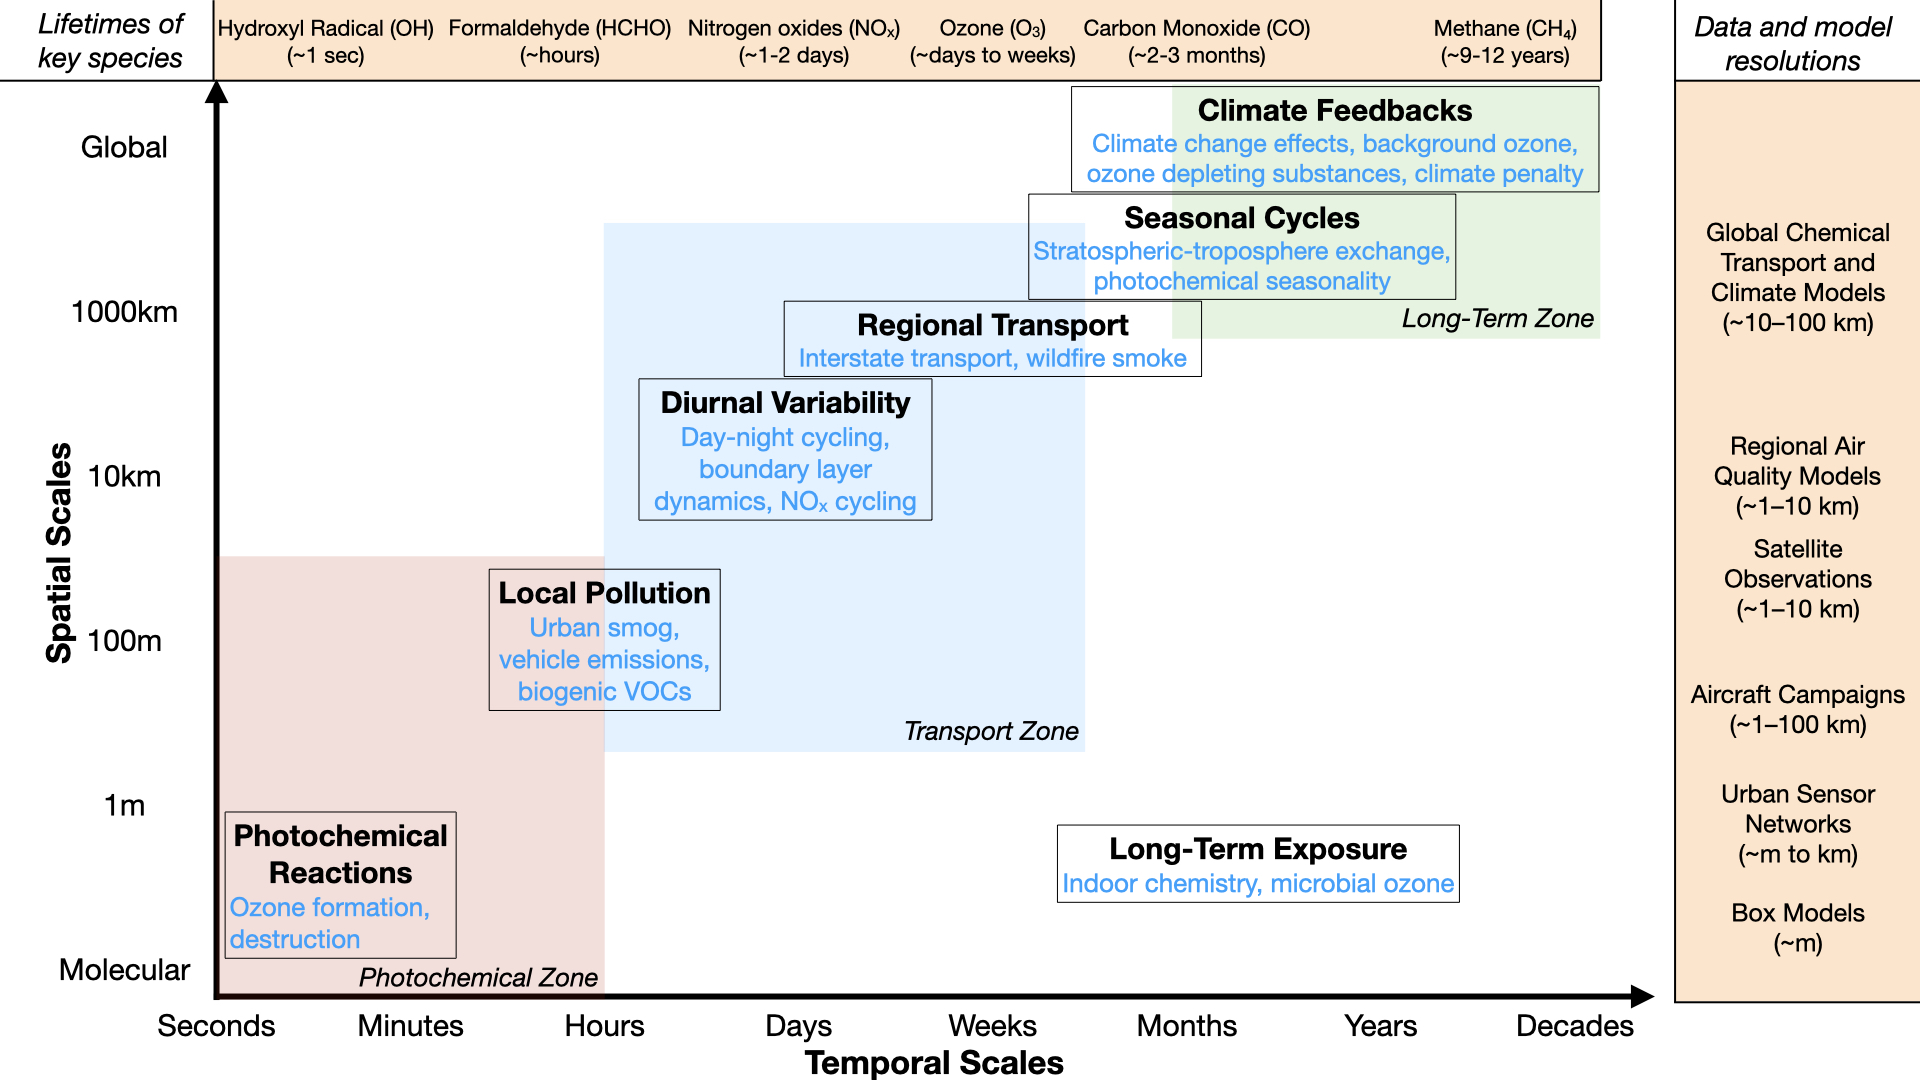
\includegraphics[width=0.85\linewidth]{figures/timeScales_Fig_ML4O3.001.png}
    \caption{Spatial and temporal scales of tropospheric ozone chemistry processes. The x-axis shows timescales, from rapid photochemical reactions to long-term climate feedbacks, and the y-axis shows spatial scales, from local pollution to global atmospheric transport. Species lifetimes and relevant data sources and models are displayed to illustrate the range and scales of phenomena and methods used to study ozone chemistry.}
    \label{fig:difficulties1}
\end{figure}


\begin{figure}
    \centering
    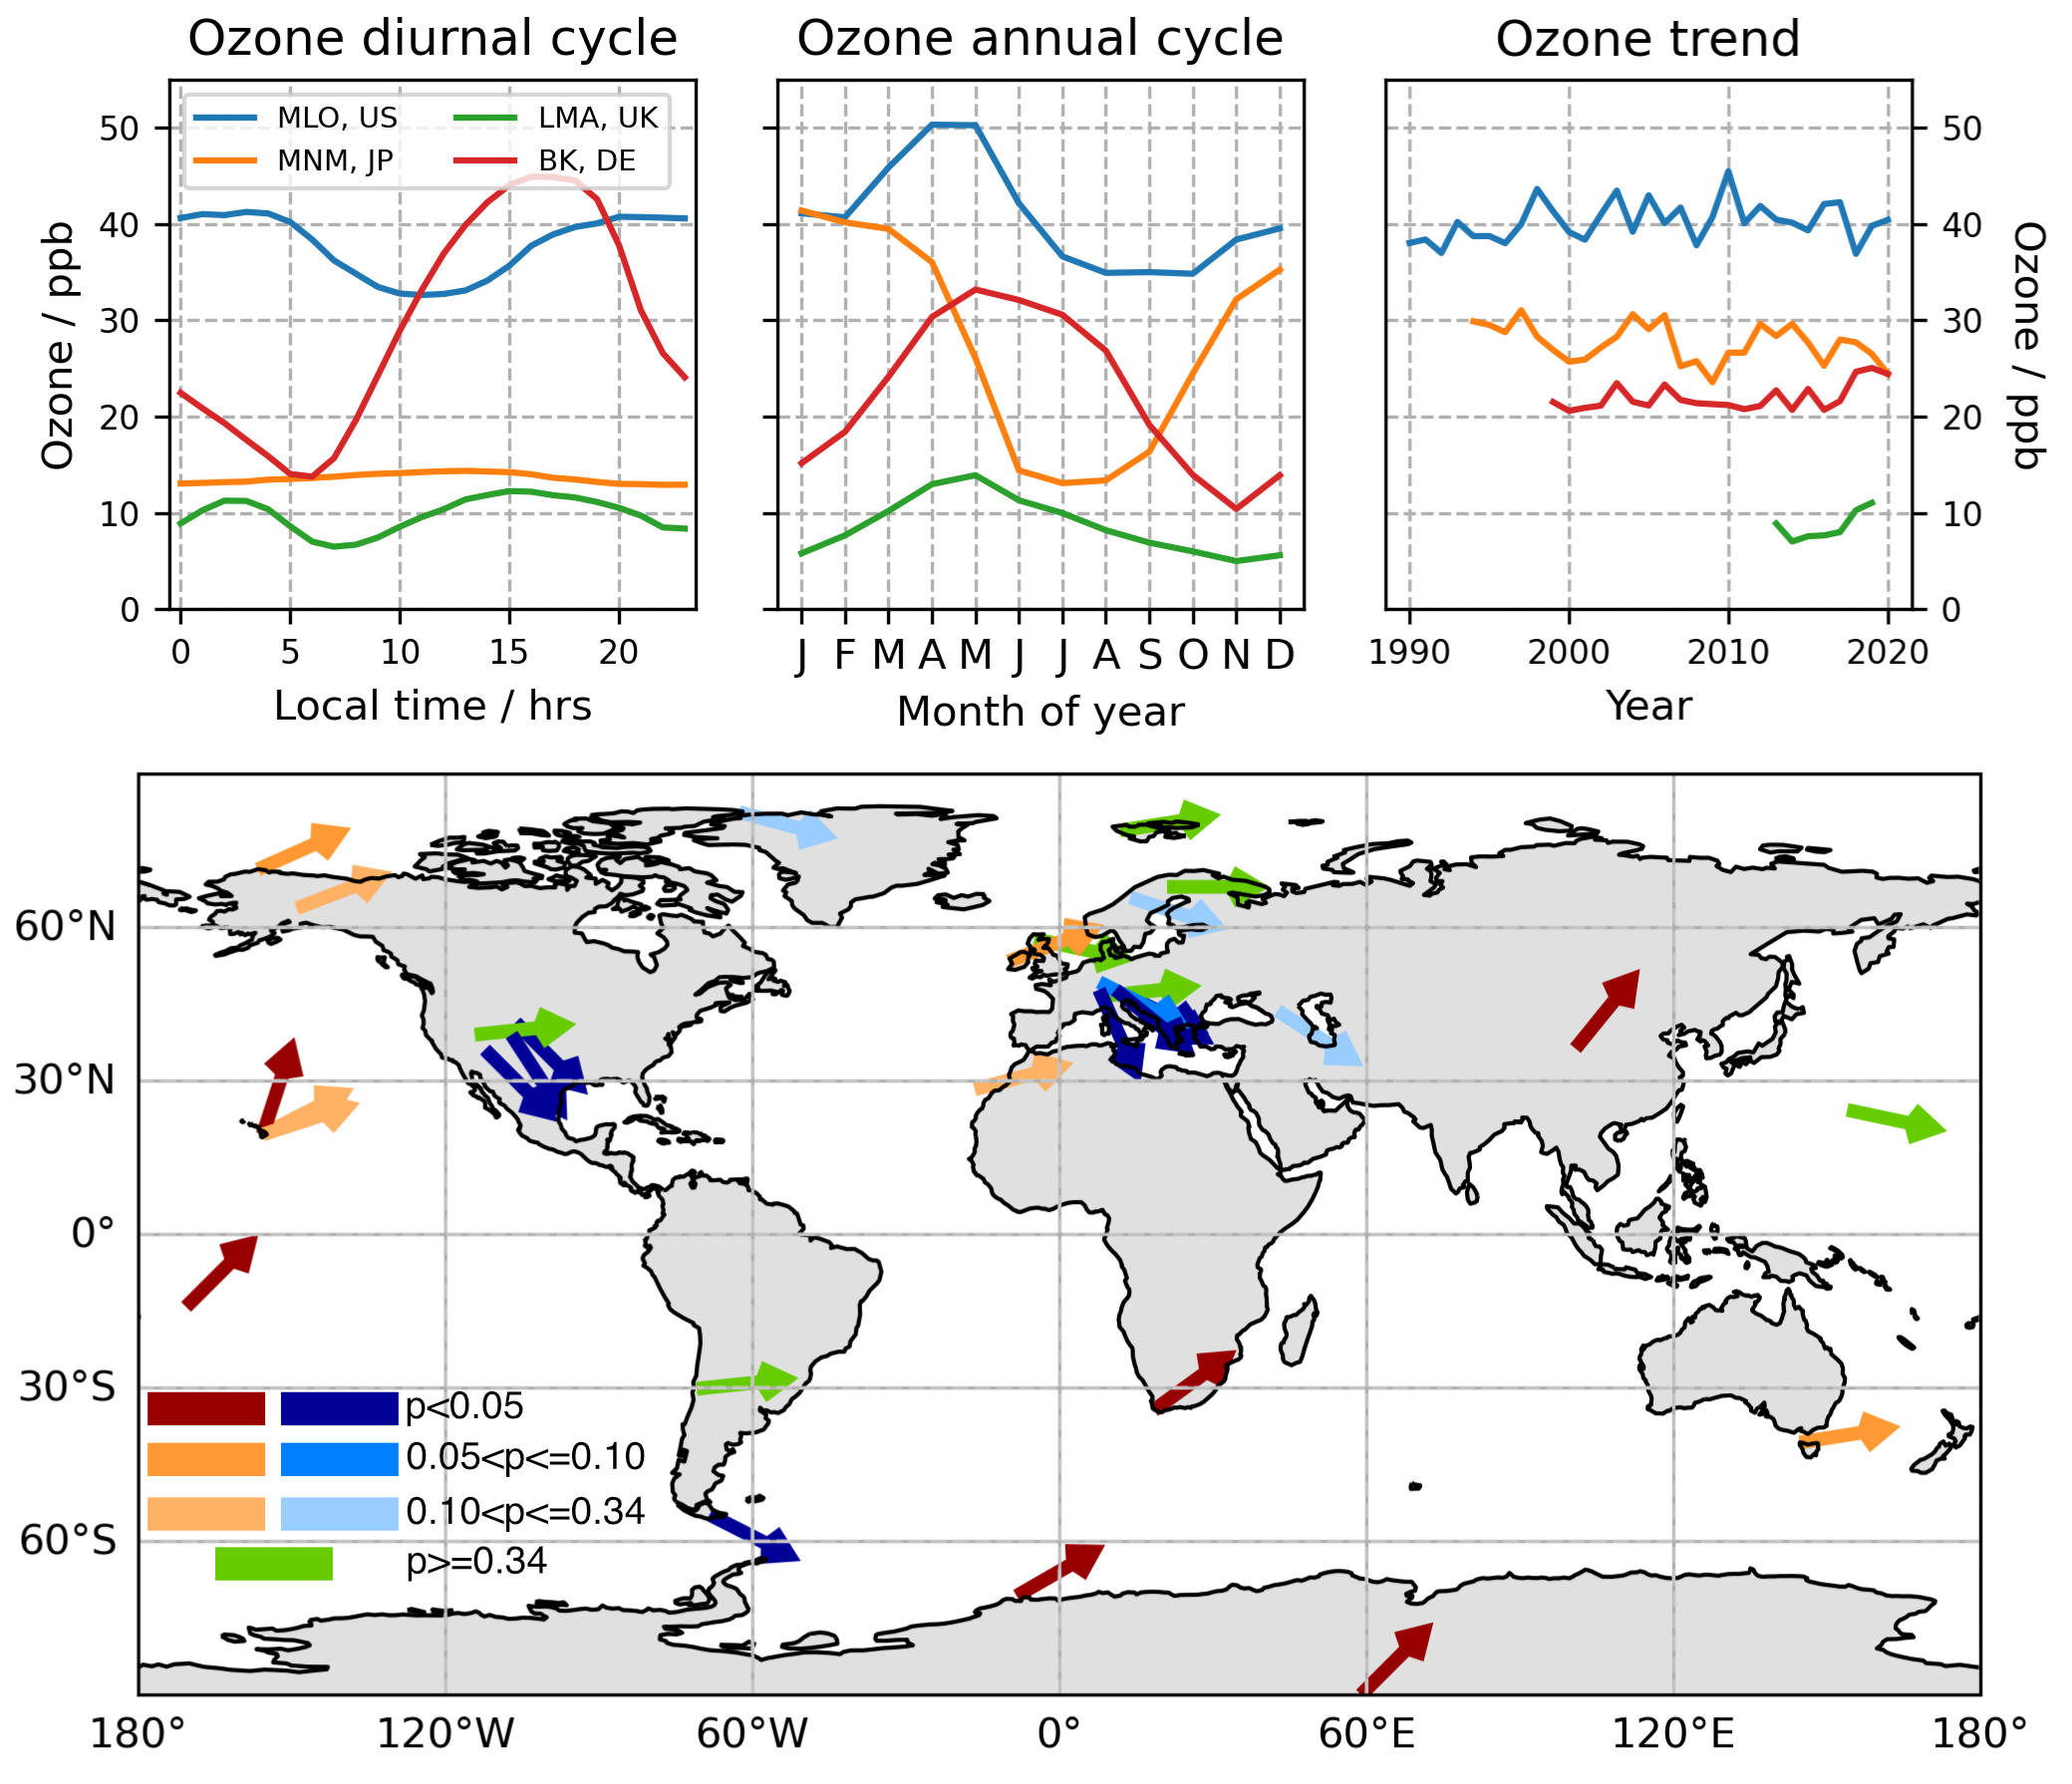
\includegraphics[width=0.7\linewidth]{figures/ozone_is_hard.png}
    \caption{Upper panel: data from the TOAR ozone database for four sites in the northern hemisphere, showing diurnal and seasonal cycles in ozone, and the long-term ozone trend. MLO, US: Mauna Loa Observatory, US; MNM, JP: Minamitorishima, Japan; LMA, UK: Marylebone Road, London, UK; BK, DE: Borken, Germany. Lower panel: long-term ozone trends based on monthly anomalies at remote surface sites. Red and blue indicate positive or negative trends respectively, with different shades giving the statistical significance of the trend at each site. Data from \citet{cooper_multi-decadal_2020} and replotted here.}
    \label{fig:difficulties2}
\end{figure}

Despite the success of ozone simulations in air quality and climate research, large uncertainties still exist in global model estimates of tropospheric ozone and its trends, although ozone is the longest- and most-measured trace gas in the observational record. Observations from ground stations, ozonesondes, and satellites indicate that tropospheric ozone has generally increased in recent decades \citep{ziemke_trends_2019, young_tropospheric_2018, IPCC_2021_WGI_Ch_2}. While global atmospheric chemistry models agree that the global tropospheric ozone burden has increased from pre-industrial times to the present day, they vary regarding the spatial distribution and magnitude of the increase \citep{skeie_historical_2020, christiansen_multidecadal_2022, fiore_understanding_2022}. Potential sources driving this model bias include uncertainties in tropical emissions \citep{zhang_contributions_2021}, nonlinear NO$_X$-VOC chemistry \citep{shah_nitrogen_2023}, stratosphere-troposphere exchange \citep{neu_tropospheric_2014}, boundary layer mixing \citep{lu_exploring_2019}, missing chemical mechanisms such as halogen chemistry \citep{wang_active_2015}, and deposition \citep{clifton_dry_2020}. 


The variation of ozone at various scales is shown in Figure \ref{fig:difficulties2}.  The figure shows the diurnal and annual cycles of ozone at four sites from the TOAR database: Mauna Loa Observatory, a Pacific mountain station, based in Hawaii, USA;  Minamitorishima, a Pacific island station in Japan; a regional continental background site, Borken, Germany, and an urban, roadside site, Marylebone Road, London, UK.  There is little consistency between the diurnal cycles at the various sites: the remote Pacific site sees little diurnal variation in ozone, but a strong seasonal cycle, with levels reaching a minimum in the summer.  In contrast, the continental, rural background site in Germany has a strong diurnal cycle, peaking in the late afternoon, and a strong seasonal cycle with a summertime maximum. The long-term trends in ozone, although weak, also vary between the sites, with both modest increases (London Marylebone Road) and decreases (Minamitorishima) being seen. The lower panel shows variation in ozone trends across the globe, ranging between -3 and 3 ppbv per year, across remote sites. These differences across ozone monitoring sites result from the complex interactions between precursor emissions, transport and chemical processes, meteorological drivers, and surface characteristics. Capturing the diversity of daily and seasonal cycles as well as trends is a key requisite of any ozone model.

\begin{figure}
    \centering
    \includegraphics[width=0.9\linewidth]{figures/In progress ML4O3_updated_DF_to_RF.png} 
    \caption{Timeline of a selection of studies using ML in ozone research (top), aligned with a selection of papers using ML in wider weather and climate modeling research (bottom). In both wider Earth system modeling research, and in ozone research there has been rapid progress over the last five years, as noted by landmark review papers highlighted in the Figure. The acronyms used are as follows. NN: neural network; RF: random forest; DL: deep learning; ML: machine learning.}
    \label{fig:timeline}
\end{figure}

Machine learning (ML) approaches, which can learn and reproduce nonlinear characteristics of a system from data \citep{hornik_multilayer_1989}, may provide a valuable complement to physical models. As the quantity and quality of observational data on ozone \citep{Schultz2017} and on the broader Earth system \citep{doi:10.1080/17538947.2016.1250829,reichstein_deep_2019} continue to grow, ML is becoming an increasingly viable tool for advancing ozone research. 

Figure \ref{fig:timeline} highlights progress in the field of ML as applied to weather and climate science, which has been rapid since the publication of the first phase of the TOAR assessment.  In their review of the state of the field of weather forecasting, \citet{bauer_quiet_2015} note many areas of progress for the field, including model throughput, the process-level detail of then current models, and the use of data assimilation techniques to improve the fidelity of the model's initial state. The impact of ML methods was not anticipated.  
\citet{rasp_deep_2018} demonstrated the potential for Deep Learning techniques to augment existing models in providing an alternative, complementary and physically consistent description of sub-grid scale processes, such as cloud microphysics.  The coupling of a fast, accurate, data-driven module, trained on finer scale simulations, to a larger scale host climate model exemplified one of the potential ways that ML approaches can contribute to the improvement of climate and weather models.  
Subsequent studies have shown in various ways the advantages of ML over traditional numerical models, particularly in terms of computational efficiency and in the ability to learn from large datasets, as demonstrated by the success of data-driven nowcasting and weather forecasting models \citep{bi_accurate_2023, lam_learning_2023, price_gencast_2024}.  

Observational data, when integrated with model simulations through data assimilation techniques, have improved the understanding of emissions and atmospheric chemistry by reducing uncertainties \citep{miyazaki_evaluation_2020}. ML can complement these efforts by combining observational data with model outputs, emulating model components, or enabling computationally cheaper simulations, thereby efficiently diagnosing sources of error in global atmospheric models and improving tropospheric ozone estimates. 
However, ML also has limitations, such as challenges in generalization, validation, and interpretability. Addressing these issues may be particularly relevant for the ozone modeling community where both predictive accuracy and physical understanding are valued.
 
In this Perspective, we provide an overview of the state of ML in tropospheric ozone research, review previous applications of ML to various problems related to ozone, and discuss persistent challenges and emerging opportunities. We highlight three areas where ML for ozone has been most widely applied: forecasts based on ground-based observations are reviewed in Section 2, methods for complementing or replacing parameterizations in numerical models of atmospheric chemistry and transport are discussed in Section 3, and ML models that are using satellite data or combined data products are presented in Section 4. Section 5 highlights and further details these cross-cutting issues and limitations with the application of ML to ozone studies, while Section 6 describes future directions for the field, highlighting emerging approaches that seek to address the cross-cutting challenges.



%%%%%%%%%%%%%%%%%%%%

\section{Applications of ML to in-situ ozone observations: short-term ground level ozone forecasting}
\label{sec:tsforecast}

\subsection{Background}
The short-term forecasting of air pollutants including ozone, i.e. predictions of expected concentrations over 1-4 days, is relevant for public health and scientific questions \citep{Buonocore2021, Hahm2021, Alari2021, Saberian2017}. State-of-the-art air quality forecasts, typically on the timescales of hours to days and up to a few days ahead, are based on the output of numerical chemical transport models (CTMs) \citep{Marecal2015}. These models may be run at higher spatial resolution for the area of interest \citep{Savage2013}, in order to better represent processes controlling air pollution at the local level, and may be post-processed to more accurately represent observations \citep{Casciaro2022}. As with other air pollutants, notably PM$_{2.5}$ \citep{Feng2015}, ML is increasingly being directly applied to the task of short-term, ground-level ozone forecasting, and to bias-correct existing air quality forecasting systems with considerable success. The availability of large and growing observational datasets has facilitated these advances \citep{Schultz2017}. However, forecasting ozone concentrations as time series with ML comes with significant challenges: forecasting ozone is a spatiotemporal problem, and ozone is controlled by processes of varying spatial and temporal scales as shown in Figure \ref{fig:difficulties1}.  

% Existing ML forecast methods are well suited to this task. Similar ML architectures and workflows have also been used to fill in missing data in observational datasets \citep{betancourt_global_2022, Wu2024}. 

Many short-term forecasting studies using ML have focused on forecasting only at selected observational stations, using observed ozone and additional chemical species, and meteorological variables where they are available from individual stations or external datasets \citep{Comrie1997, cobourn_comparison_2000, Kolehmainen2001,Eslami2020, sayeed_novel_2021, leufen_o3resnet_2023, Hickman2023}. Furthermore, since it is difficult to downscale a relatively coarse CTM at specific locations, using time series data from a particular station is an attractive way to make predictions at particular locations. However, approaches of this kind do not necessarily provide ozone forecasts across all locations that may be of interest, as a gridded model product model might.

\subsection{Progress and State of the Science}

As with other fields, the advances in ML-based ozone forecasting have been pushed by developments on two axes - first, increasing quantities of data and second, larger models with more appropriate inductive biases. The field has a long history (see Figure \ref{fig:timeline}), with studies being published even during the most recent artificial intelligence (AI) "winter", beginning with a feed-forward neural network (NN) in 1996 \citep{Yi1996}. \citet{Comrie1997} illustrated that a NN could be used to forecast ozone at eight stations in the USA. This was followed by further feed-forward NN approaches, often with datasets drawn from a single location or city \citep{cobourn_comparison_2000, Kolehmainen2001}. Neural methods were typically evaluated in comparison with (autoregressive) regression models, often finding that NNs were better able to forecast ozone concentrations and extrema on test data \citep{Nunnari1998, Schlink2003, Chaloulakou2003}, although the improvement was often only marginal. Alongside the successes of feed-forward NN architectures, other work drew attention to methods seen to be more interpretable, such as fuzzy logic systems and regression trees \citep{Gardner2000, heo_new_2004}. Further work leveraged methodological advances in ML architectures designed for temporal data, including the use of recurrent neural networks (RNNs) and convolutional neural networks (CNNs) to account for lagged relationships in the time series data \citep{Eslami2020, sayeed_novel_2021, Kleinert2021}. Recent work has combined architectures to model the relationships that control ozone, including combining components such as transformers and CNNs to account for the temporal and spatial information relevant to forecasting \citep{Chen2022, cheng_spatio-temporal_2022, han_capability_2023}. However, datasets have typically been limited to single countries or cities, due to the lack of a combined database of station measurements. The introduction of the TOAR surface database \citep{Schultz2017} and the TOAR-II database have facilitated recent studies on data drawn from multiple countries \citep{leufen_o3resnet_2023, Hickman2023}. The importance of the curation of large datasets for scientific progress in ML is highlighted in the Outlook section. 

Increasingly, more complex architectures are being used to enhance the accuracy of ozone forecasts, and more data are being included as input to the models. The inputs that are relevant to the physical drivers of ozone concentrations, such as past observations of ozone and covariates, and nearby covariates, reflect processes that control ozone observations, and feasibly contribute to improved ozone forecasting and infilling. Recently, methods on the scale of the ML architectures and data used for weather forecasting \citep{bi_accurate_2023, lam_learning_2023} have been transferred to ozone forecasting by leveraging very large datasets and models. In weather studies there is work on forecasting at observation stations using these methods, and transferring these methods to forecast ozone at ground-level stations is feasible \citep{manshausen_generative_2024}. 


% \subsection{Future Outlook}

% While forecasting ground-level ozone has seen some successes, there are still some necessary steps before we have reliable operational ML forecasts. As in other fields, the community has seen improved performance with scaling datasets, and training across a variety of environments with rich data \citep{leufen_o3resnet_2023}. While the TOAR database of surface observations provides a large collection of in-situ data, the community is still missing a fused, global and gridded benchmark dataset that could be used to robustly compare methods \citep{Dueben2022, Rasp2024}, and explore model deficiencies. Creating this dataset should be a collaborative effort that may provide the step-change in ground level air pollution forecasting that other benchmark datasets have precipitated in other fields \citep{Deng2009}. Part of this benchmark should focus on extreme events and probabilistic metrics, as currently the community does not evaluate performance on extremes thoroughly, and encouraging probabilistic models and metrics may improve performance on extremes. While generalization is less of an issue for short-term forecasting, building models that can generalize to undersampled regions of the world would facilitate better pollution forecasting in countries with fewer data. Finally, work on interpretability and explainability is limited, and further study may give more insight into the internal working of these models, and possibly insight into physical processes.


\section{Applications of ML methods in atmospheric chemistry modeling}
\subsection{Background}
Global modeling of atmospheric chemistry is a grand computational challenge due to the high dimensionality of coupled chemical species, the nonlinearity and numerical stiffness of solving chemical mechanisms, and interactions with transport on all scales. The inclusion of comprehensive atmospheric chemistry in Earth system models (ESMs), which simulate the interactions between the atmosphere, oceans, land surface, and biosphere, is a priority science frontier \citep{national_research_council_national_2012}. Atmospheric chemical mechanisms are typically implemented in CTMs, which focus on the distribution and chemical evolution of species in the atmosphere. For some applications, chemistry-climate models (CCMs) may also couple chemical processes with climate dynamics, allowing feedback between chemistry and climate. Current atmospheric chemistry models integrate the coupled chemical kinetic equations for mechanism species over model time steps using high-order implicit numerical solvers, but these solvers are computationally expensive \citep{sandu_benchmarking_1997} and often dominate the cost of an atmospheric simulation \citep{eastham_geos-chem_2018}. Such costs put the inclusion of atmospheric chemistry in tension with other computationally intensive ESM/CCM priorities such as increased spatial resolution and ensemble simulations. The current slowdown in the rate of increase in the speed of computer CPUs—the “end of Moore's law”—underscores the need for computationally efficient approaches \citep{theis_end_2017}.
 
Chemical solvers in atmospheric models compute the local evolution of species concentrations over a chemical time step that may range from minutes to hours depending on the model \citep{brasseur_modeling_2017}. The chemical mechanisms used in regional to global atmospheric models and ESMs typically include $\mathcal{O}(100)$ coupled species with chemical lifetimes ranging from less than a second to much larger than the model time step. High-order implicit solvers can integrate this system of stiff coupled differential equations with high accuracy and fast implementations of these schemes are available, but they are still extremely costly for atmospheric models. Atmospheric models may combat that cost by decreasing the size of the chemical mechanism, breaking down the stiffness of the problem, or using lower-order approximations. However, these methods rarely achieve a speedup of more than a factor of two \citep{lin_adaptive_2023, shen_adaptive_2020} and sometimes lead to loss of accuracy in the model results. As a consequence, these computational barriers limit the ability for high-resolution simulations, prevent detailed uncertainty analyses, and complicate the coupling of atmospheric chemistry into CCMs/ESMs for long-term climate simulations without significant compute resources. 
 
ML methods could be transformative in this area for both reducing the cost of an atmospheric chemistry simulation and facilitating their incorporation into ESMs. ML methods seem well-suited to replace chemical solvers in atmospheric models because the chemical computation is very repetitive, involving the integration of similar conditions in neighboring grid cells and successive time steps. However, the large number of coupled species brings a ‘curse of dimensionality’ to the problem, and ML methods have no check on error growth, unlike in standard chemical solvers where errors are dampened by the negative response to perturbations (Le Chatelier’s principle).
                                                 
% There are a variety of examples using output from CTM and air quality models in tandem with satellite measurements, ground-level monitoring observations, meteorological reanalysis data, and emissions databases to predict or improve forecasts of ozone. These improvements can be achieved through various methods, including data fusion techniques and the creation of reduced-order models. However, because such studies involve additional data besides model outputs, they will be discussed in other sections (Sections 2 and 4). Here, we emphasize studies primarily employing data from atmospheric chemical models.

\subsection{Progress and State of the Science}
Largely, ML methods in atmospheric chemistry modeling currently involve emulating model components to improve model parameterizations, reduce computational bottlenecks, and create simplified, reduced-order models. Here, emulation refers to an ML model reproducing the same calculations as a component of a complex physical or simulated system for a set of inputs. There exists a growing number of studies forecasting ozone on short- (hourly) \citep{yafouz_comprehensive_2022} and longer-term \citep{du_forecasting_2022, Chen2023} timescales, spanning from city- \citep{ojha_exploring_2021} to regional-level \citep{ortiz_combination_2021} spatial scales. However, few of these studies have been implemented in operational settings (i.e., within CTMs, CCMs) to offer insight beyond that of traditional model-to-observation comparison methods.   

\subsubsection{Offline ML and reduced order modeling}
\citet{Xing2020} used a hierarchy of ML models containing a CNN and long short-term memory (LSTM) network to predict ozone concentrations from CMAQ model output over 7-day forecast periods. \citet{kuo_ozone_2023} investigated how accurately ML models can learn the ozone-NO$_X$-VOC chemical relationships in a chemical mechanism and found that their ML model produced distorted NO$_X$ and VOC-limited isopleths when only trained on CMAQ model outputs. \citet{kelp_toward_2020} trained an NN integrator in a photochemical box model, including an encoder/decoder to decrease dimensionality, and a recursive feedback loop over 24-hr integration time to control error growth. They found that they could compress the 101-species dimension of their mechanism into 16 features without significant error penalty and avoid error growth within a selected time horizon, though error increases beyond this window. \citet{yang_atmospheric_2024} created an ML surrogate for a low-dimensional (11 species) chemical box model that both compresses the dimensionality of the chemical mechanism and reduces the numerical stiffness of the problem. They achieve numerical stability within a 9-day training window but acknowledge that such an approach may be difficult for more complex and higher-dimensional chemical mechanisms. \citet{liu_neural_2024} employed a Fourier Neural Operator with time-embedded attention to calculate chemical concentration changes as a learnable time-dependent process. They achieved higher accuracy metrics compared to standard neural operators and U-Nets in simple box model-like simulations. 

\subsubsection{Online ML within global models}
While there is a growing literature on using ML to emulate and improve the representation of atmospheric processes, few have implemented these ML models online within CTMs/ESMs to evaluate their effectiveness. \citet{keller_application_2019} created a random forest (RF) integrator for the GEOS-Chem global 3-D CTM driven by re-analyzed meteorological data. They achieved successful short-term simulations but found large error growth after a few weeks. \citet{liu_correcting_2022} developed a gas-phase NN solver for the CMAQ regional CTM over China, combining a standard implicit solver for radicals and oxidants with an ML solver for VOCs. They achieved an order of magnitude speedup over a 1-month simulation but with error growth over remote ocean grid cells. \citet{shen_machine-learning-guided_2022} used an unsupervised ML algorithm (simulated annealing) to create submechanisms of the full chemical mechanism in GEOS-Chem for which they solve the coupled kinetic system only for the fast species in the submechanism. The computational cost of the chemical integration decreased by 50\% and the relative difference in ozone was <0.5\% in the troposphere and <0.1\% in the stratosphere over 8-year simulations. \citet{kelp_online-learned_2022} implemented the low-dimensional “Super-Fast” chemical mechanism in GEOS-Chem using online training of the ML emulator, achieving stable 1-year simulations for ozone prediction with less than 10\% bias compared to the reference and reducing computational cost by a factor of five. However, their ML solver had relatively lower accuracy in pristine marine regimes with lower chemical concentrations. \citet{xia_advancing_2024} implemented a self-attention transformer chemical solver online into the WRF-Chem CTM achieving an eight-time speedup over the conventional solver with stable bias metrics for 74 species. Their approach shows promise for accurate predictions of chemical concentrations with low overhead when coupling the ML solver to the CTM, but simulations were only run for 15 days and stability over longer time scales (>1 year) remains to be seen. 

While ML models are typically trained and deployed using Python libraries, integration of these models into CTMs remains limited because CTMs are written in Fortran, which cannot natively call Python. Current solutions include rewriting models in neural Fortran \citep{keller_application_2019}, using the C Foreign Function Interface (CFFI) to create C-style bindings for Python scripts \citep{kelp_online-learned_2022, zhong_wrfml_2023}, or packaging ML models as callable static or dynamic libraries using TorchScript and LibTorch \citep{xia_advancing_2024}. Depending on the architecture and complexity of the coupled ML model, all coupling methods result in a speedup over the conventional reference solver \citep{de_burgh-day_machine_2023}.

\subsubsection{ML modeling processes affecting ozone chemistry}
A number of ML and data-driven advances have been made for CTM modeling that are separate from creating an ML chemical solver. \citet{wiser_amore-isoprene_2023} and \citet{wang_implementation_2023} created automated chemical mechanism reduction approaches to reduce the high dimensionality of the VOC precursors of ozone and secondary organic aerosol. \citet{sturm_conservation_2022, sturm_mass-_2020} developed methods to enforce mass and stoichiometric conservation rules in outputs from ML emulators. \citet{anderson_machine_2022} used gradient-boosted regression trees to develop a parametrization for the OH radical, a key driver of ozone formation, for CCM models. Similarly, \citet{zhu_combining_2022} trained an ML model on CTM output parameters and satellite observations from OMI to predict urban OH concentrations. \citet{huang_neural_2022} created an NN-assisted Euler integrator to speed up the iterative computations within an implicit solver routine. 

There is a growing literature on ML approaches for bias corrections on existing air quality modeling systems \citep{Neal2014, Borrego2011, Silibello2015}. These approaches generally learn the error between the output of a numerical model and some observations and then apply this error correction to the output of the numerical model. \citet{silva_deep_2019} developed an ML parameterization for ozone dry deposition velocities using surface observations that outperformed those within CTMs for certain locations. Similarly, \citet{ivatt_improving_2020} created an eXtreme Gradient Boosting (XGBoost) model trained on ozone surface observations and data from ozonesonde networks to predict and correct GEOS-Chem model biases. \citet{liu_correcting_2022} developed a NN model to correct surface ozone in the UKESM model, finding that temperature drives biases over Northern Hemisphere continental areas while photolysis rates contribute to global ozone biases. \citet{nowack_using_2018} used a hierarchy of ML methods to build temperature-based ozone parameterizations for climate model sensitivity simulations. \citet{colombi_why_2023} used RFs to remove the effect of weather coupled to ozone trends. \citet{Gouldsbrough2024} used a gradient-boosted tree to downscale ozone model output from the EMEP4UK CTM. \citet{ye_diagnosing_2022} used an RF model to identify underlying causes of CTM bias in simulating daily surface ozone variability, finding that CTM underestimates in the dry deposition velocity and cloud optical depth on wet/cloudy days were the primary drivers over China. 
 
\citet{park_learned_2023} created a prototype ML discretization for a one-dimensional horizontal passive scalar advection, an operator component common to all CTMs, and achieved stability and orders of magnitude computational gain relative to the reference when coarse-grained. \citet{sturm_advecting_2023} developed a data-driven compression method for chemical tracers within a CTM and advected the compressed representation, achieving a computational gain of 1.5$\times$ without loss of accuracy. There have been developments of ML emulators in box models for organic aerosol mechanisms detailing the ML models’ accuracy with respect to interactions with ozone \citep{mouchel-vallon_toward_2023, schreck_neural_2022}. The photolysis frequencies used to inform ozone concentrations, calculated from the radiative transfer components of atmospheric models, can themselves be emulated using NNs \citep{lagerquist_using_2021} and have the longest relative history of ML emulation for atmospheric modeling \citep{krasnopolsky_new_2005,krasnopolsky_decadal_2008}. 

% \subsection{Future Outlook and Priorities}

 The near-term future of integrating ML with 3-D atmospheric chemistry and climate modeling relies on understanding the uncertainties and limitations of ML emulation. Such knowledge is essential for improving or approximating specific chemical parameterizations rather than attempting to replace full-scale, multiscale chemistry simulations. Key priorities include incorporating ML models into CTMs, CCMs, and ESMs, as well as characterizing their behavior over extended time scales (>1 year). While short-to-seasonal scale emulation may be suitable for forecasting horizons, it offers limited applicability for integrating comprehensive atmospheric chemistry into climate simulations. %Additional priorities should include scaling regional ML models to a global context and identifying the strengths of ML (e.g., speed of operation, pattern recognition of high volumes of data) alongside its weaknesses (e.g., inability to approximate multiscale dynamics, instability over time, resource-intensive training and black box nature). 

% In the context of using ML for model component emulation and replacing traditional components, a major challenge is managing coupled instabilities, where ML predictions accumulate errors and drift from the reference model over time. This instability is also prevalent in ML-based model emulation for weather and climate applications. Consequently, ML approaches are increasingly employed to develop end-to-end models that process raw input data (e.g., emissions, meteorological fields) and directly predict outputs such as ozone concentrations. While end-to-end models bypass the challenges of emulating individual components and are less prone to short-term instabilities and operator splitting issues, they also limit the ability to track uncertainty metrics tied to physical parameters and processes. 

% Another emerging area is the use of Physics-Informed Neural Networks (PINNs), which embed physical laws into an ML model’s architecture. While ML has been used to emulate traditional numerical solvers, this approach has often sacrificed accuracy and stability over long-term timescales in exchange for faster computations. Traditional solvers, though computationally expensive, do not exhibit these error instabilities (see Le Chatelier’s principle). PINNs may offer a solution to balance speed with accuracy and have shown success in smaller-scale systems, such as single ODEs or PDEs \citep{karniadakis_physics-informed_2021}. Although their application to large groups of ODEs in atmospheric chemistry has not yet been widely explored, PINNs may hold the potential for achieving greater accuracy than traditional solvers, possibly overcoming some of the limitations of ML approaches in atmospheric chemistry modeling. However, PINNs may not enforce physical laws perfectly and the inherent black-box nature of certain ML components limits their transparency compared to physical models, which provide clearer constraints. Therefore, while PINNs may address some computational challenges, their contribution to advancing process-level understanding in atmospheric chemistry remains uncertain.

% At present, there are underexplored opportunities to merge the current successes in ML weather and climate model emulation with CTMs. Thus far, atmospheric chemistry data have been largely excluded from ML weather and climate applications, as these current supervised learning frameworks are typically non-extensible, requiring retraining of the entire ML model when incorporating new chemical information. In contrast, unsupervised learning model frameworks, such as large-scale, pre-trained ML architectures called foundation models (discussed in greater detail in Section 6) or Large Language Models (LLMs), can identify patterns or clusters in data without explicit labels, offering a new frontier for ingesting and potentially improving ML modeling of atmospheric chemistry. These foundation models, such as Aurora \citep{Bodnar2024} , an ML weather model, can be 'fine-tuned' on CTM data: a process where a pre-trained ML model is further trained on a smaller, specialized dataset to improve its performance on a specific domain at a lower computational cost. The Aurora model is fine-tuned on a subset of six criteria pollutants, including ozone, from the Copernicus Atmosphere Monitoring Service (CAMS) reanalysis dataset. Fine-tuning ML weather and climate models enables the addition of chemical species to an ML model that is already trained on atmospheric dynamics. However, adding chemical species such as VOCs to Aurora in the absence of emission inputs (which these foundation models currently do not consider) on the model's native 6-hour forecast time steps likely presents challenges. Greater emphasis is needed on understanding the factors influencing ML model performance, whether stemming from the ML model architecture, the quality and curation of training data, or uncertainties inherent in the physical processes of emissions, transport, and chemistry. 

\section{Applications of AI/ML methods to satellite observations}

\subsection{Background}
Satellite measurements provide detailed information on the spatiotemporal distribution of atmospheric composition and related parameters, such as those associated with surface air quality. Satellite measurements have greater spatial and temporal coverage compared to in-situ observations and they can fill the gaps in those sparse distributions, particularly in remote areas where in-situ observations are not available. 

Over the past few decades, multiple satellites have been launched to measure total ozone columns. %, including the Total Ozone Mapping Spectrometer (TOMS) \citep{prospero_environmental_2002}, Scanning Imaging Absorption Spectrometer for Atmospheric Cartography (SCIAMACHY) \citep{bovensmann_sciamachy_1999}, Ozone Monitoring Instrument (OMI) \citep{veefkind_total_2006}, Global Ozone Monitoring Experiment (GOME) \citep{coldewey-egbers_total_2005}, GOME-2 \citep{loyola_gome-2_2011} and the Sentinel-5P Tropospheric Monitoring Instrument (TROPOMI) \citep{garane_tropomis5p_2019}. Geostationary satellite observations, such as the Tropospheric Emissions: Monitoring of Pollution (TEMPO) \citep{Naeger2021} and Geostationary Environment Spectrometer (GEMS) \citep{baek_evaluation_2023} observe detailed spatial and temporal patterns of total column ozone and other air pollutants.
However, total column measurements cannot be used to provide insight into near-surface ozone because the amount of stratospheric ozone is much larger than the amount of tropospheric ozone. Tropospheric ozone information has been directly retrieved using measurements from nadir-viewing thermal infrared (TIR) sounders, such as the Tropospheric Emission Spectrometer (TES) \citep{bowman_capturing_2002} and the Infrared Atmospheric Sounding Interferometer (IASI) \citep{boynard_measurements_2009}, and by combining measurements from both ultraviolet (UV) and visible (VIS) wavelengths by the Tropospheric Emissions: Monitoring of Pollution instrument \citep{johnson_evaluation_2018}. In addition, the limb-nadir matching method employs stratospheric ozone data from limb-viewing measurements, such as those from the Microwave Limb Sounder (MLS), to derive tropospheric columns from observed total columns \citep{ziemke_trends_2019}. Recently, multispectral satellite approaches, such as IASI and the Global Ozone Monitoring Experiment (GOME) 2 \citep{cuesta_transboundary_2018} and TES and the Ozone Monitoring Instrument (OMI) \citep{colombi_new_2021}, have been implemented to derive tropospheric ozone profiles with increased sensitivity to the lower troposphere.  

Nevertheless, satellite observations of ozone are still limited in spatial, temporal, and vertical resolution and are not sufficiently sensitive to ground surface levels. On the other hand, measurements of precursors, such as NO$_2$ and CH$_2$O from OMI, GOME-2, the Tropospheric Monitoring Instrument (TROPOMI), and the Ozone Mapping and Profiler Suite, have provided unprecedented information to assess the formation processes and surface concentrations of pollutants such as ozone and aerosols. Despite these advancements, technical challenges remain in accurately assessing near-surface air pollutant concentrations from satellite observations of precursors. ML techniques can be used to fill the gaps in the information available from satellite observations and to improve the estimation of surface air pollutants.

\subsection{Progress and State of the Science}

ML has been widely used in satellite applications, especially in remote sensing imagery \citep{maxwell_implementation_2018} in the past and is becoming more widely applied to atmospheric composition data. ML has been applied to satellite observations in two main categories: (1) to generate atmospheric concentration retrievals and blend multi-satellite products, and (2) to fill gaps in observational information, including surface concentrations and emissions estimates. 

\subsubsection{ML models for fast retrievals and multi-satellite blending}

Ozone retrieval is the task of estimating ozone profiles from spectrometers on satellites, which measure radiance spectra from the atmosphere. ML-driven retrieval algorithms have emerged as a powerful tool to improve the processing efficiency of atmospheric composition satellite products. Traditional physics-based retrievals, which are based on radiative transfer models (RTMs) and solve their inverse problem, have been widely used to generate satellite profiles of atmospheric composition concentrations -- known as level 2 (L2) products -- from observed spectral radiances. They consider detailed atmospheric processes to retrieve concentrations, but are computationally expensive. To speed up the retrieval processes, numerical inversion schemes have been replaced by ML algorithms that are trained using RTM inversions. Such an approach has been applied to satellite measurements to retrieve ozone \citep[e.g.,][]{muller_ozone_2003}, SO$_2$ \citep[e.g.,][]{li_new_2022}, isoprene \citep[e.g.,][]{wells_next-generation_2022}, and CO$_2$ \citep[e.g.,][]{xie_fast_2024}. 

In addition, ML techniques have been used to correct for satellite product bias and blending multiple products. For example, \citet{oak_bias-corrected_2024} corrected the Geostationary Environment Spectrometer operational L2 NO$_2$ vertical column density  with a ML model to match more mature TROPOMI observations, while preserving the GEMS data density. Similarly, \citet{balasus_blended_2023} created a blend of TROPOMI and Greenhouse Gases Observing Satellite (GOSAT) methane products obtained by training the ML model to predict differences between TROPOMI and GOSAT co-located observations. \citet{shi_harmonizing_2024} developed an ozone column harmonization method using ConvNeXt \citep{liu_convnet_2022} to learn a mapping between OMI and TROPOMI, creating a reconstructed ozone column product with the long length of OMI availability and high spatial resolution and accuracy characteristics of TROPOMI. Such bias correction and blending approaches are powerful for providing accurate and consistent datasets for various science applications, for example, emissions inversion. 

\subsubsection{Fill in gaps in observational information }

ML can also be used to fill gaps in observational information, such as supplementing missing data due to clouds to provide a continuous spatiotemporal distribution, and providing surface quantities that cannot be directly measured by satellites. Satellite observations of ozone and its precursors, combined with additional information such as meteorological conditions, land-use, population density, and anthropogenic emission inventories, have been used in NN or RF models to estimate spatiotemporal patterns of surface ozone concentrations at high spatial resolutions in different regions of the world \citep{di_hybrid_2017, wang_machine_2022, zhu_combining_2022, kang_estimation_2021, ghahremanloo_deep_2023}.

\citet{di_hybrid_2017} proposed a hybrid NN model using data from OMI, GEOS-Chem CTM outputs, ozone vertical profiles, meteorological variables, land-use terms and other atmospheric compounds to predict
daily maximum 8-hour average (MDA8) ozone in the continental United States. XGBoost was used by \citet{liu_spatiotemporal_2020} to predict MDA8 ozone with similar inputs, while \citet{jung_machine_2024} used XGBoost with OMI and MODIS products to estimate MDA8 at 1km resolution in Taiwan. \citet{ghahremanloo_deep_2023} used a CNN with TROPOMI data as an input to estimate MDA8 in the United States. Among various ML techniques, \citet{zong_deep_2024} concluded that Deep Forest performs better than other shallower, tree-based regression models to estimate surface ozone from satellite ozone products. Similar surface concentration estimations based on NN or RF models have been applied to satellite NO$_2$ products to estimate surface NO$_2$ concentrations with high spatial resolution \citep{kim_importance_2021}, and to satellite aerosol optical depth measurements to estimate surface PM$_{2.5}$ concentrations \citep{huang_high-resolution_2021, xiao_evaluation_2021} which are useful for exposure estimates.

Emissions estimation using satellite observations of atmospheric composition concentration is another important ML application. ML techniques have been applied to improve the computational efficiency and accuracy of emissions estimation at various scales compared to traditional approaches based on data assimilation and other approaches \citep{dadheech_high-resolution_2024, xing_rapid_2022, tu_estimation_2023, li_emission-based_2024, bruno_u-plume_2024}. 

In addition, ML-based anomaly detection methods pinpoint pollution hotspots, such as urban centers and areas of high industrial activity. For instance, \citet{joyce_using_2023} developed a deep NN to identify and quantify point source emissions of methane from hyperspectral images from the PRecursore IperSpettrale della Missione Applicativa (PRISMA) satellite with 30 m spatial resolution. ML models can also identify contributions from various emission sources (e.g., traffic, industry, wildfires) \citep{kang_mitigating_2024, finch_automated_2022, kurchaba_anomalous_2023, rollend_machine_2023}. 

ML can also be used to characterise key chemical environments and classify each area into different chemical regimes based on satellite observations of pollutants and their precursors. For example, the abundance of OH in urban areas initiates the removal of pollutants, making it a key species to describe the urban chemical environment. Despite its importance, it cannot be measured at the regional scale due to its very short chemical lifetime \citep{duncan_opinion_2024}. 

% \citet{zhu_combining_2022} developed a ML approach as an efficient alternative to computationally expensive CTM-based OH simulations, using observations of tropospheric NO$_2$ and HCHO columns from OMI as input to a ML model to predict daily near-surface OH. \citet{anderson_technical_2023} used a combination of ML models, CTM simulations, and various satellite observations to estimate tropospheric column OH in the tropics over the open oceans. They also showed that systematic biases in satellite products such as NO$_2$ may lead to biases in OH estimation.

These results indicate that combining satellite observations with ML approaches can provide important information for understanding and improving air pollution, including surface ozone and its precursor emissions, which cannot be directly measured from satellite observations. Further progress in this area can be expected through careful evaluation and understanding of the characteristics and quality of satellite products, selection of effective supplementary information, and further development of appropriate ML methods.


%\subsection{Future Outlook and Priorities}

%As with the integration of ML with atmospheric chemistry 3-D modeling, priorities in the domain of ML with remote sensing should focus on the movement from regional to globally generalizable models. Remote sensing datasets are largely available on a global scale, but ML models in this context are limited due to lack of adequate ground truth. The inclusion of tropospheric ozone domain experts is critical for the correct evaluation of models where ground truth is not available to assess performance as compared to CTMs. 

%Satellite observations are available at regional and global scales, for temporal scales ranging from hourly to decadal scales. As with the integration of ML with CTMs, priorities in the area of ML using satellite observations need to be further focused on their appropriate application at various spatio-temporal scales. With  increasing resolution of satellite observations, the generalization of methods for producing satellite retrievals by ML has also become one of the priorities of the community.

%Each satellite measurements have different characteristics, and data quality may vary not only spatially but also temporally. In many areas, especially in developing countries where air pollution is severe, ground truth observations are not available, hindering the application and validation of ML models. Careful validation of ML results is desirable, for example, taking into account the differences in spatial representativeness between satellite and ground-based observations. Another important challenge is how to integrate and use the results of validation using independent observations and uncertainty information from satellite retrievals as input for ML.

%As the satellite constellation continue to evolve, data fusion of multiple instruments and multiple species using ML, in addition to chemical reanalysis approaches using data assimilation techniques \citep{inness_cams_2019, miyazaki_updated_2020}, will play an important role in achieving consistent analysis of long-term trends. Combining satellite data with ML offers a further approach to investigate the linear and non-linear processes controlling air pollutant dynamics, complementing ground-based measurements and CTM estimates.

%%%%%%%%%%%%%%%%%%%%

\section{Challenges and Limitations}

In this section, we reflect on some common challenges and limitations of using ML in the context of ozone forecasting, modeling, and observations (Figure \ref{fig:sankey}). While we describe many challenges which are shared with ML for physical modeling in general, we also highlight challenges specific to ozone modeling with ML in the following sections. In particular, we describe challenges related to the diversity and spatial heterogeneity of ozone monitoring datasets, the difficulty of modeling chemical processes operating at different timescales and with limited data on factors influencing ozone concentrations, as well as detailing challenges more generally applicable to ML for physical modeling. Furthermore, in this section and the next, we propose concrete next steps to make progress on those challenges specific to ozone. 

\begin{figure}
    \centering
    %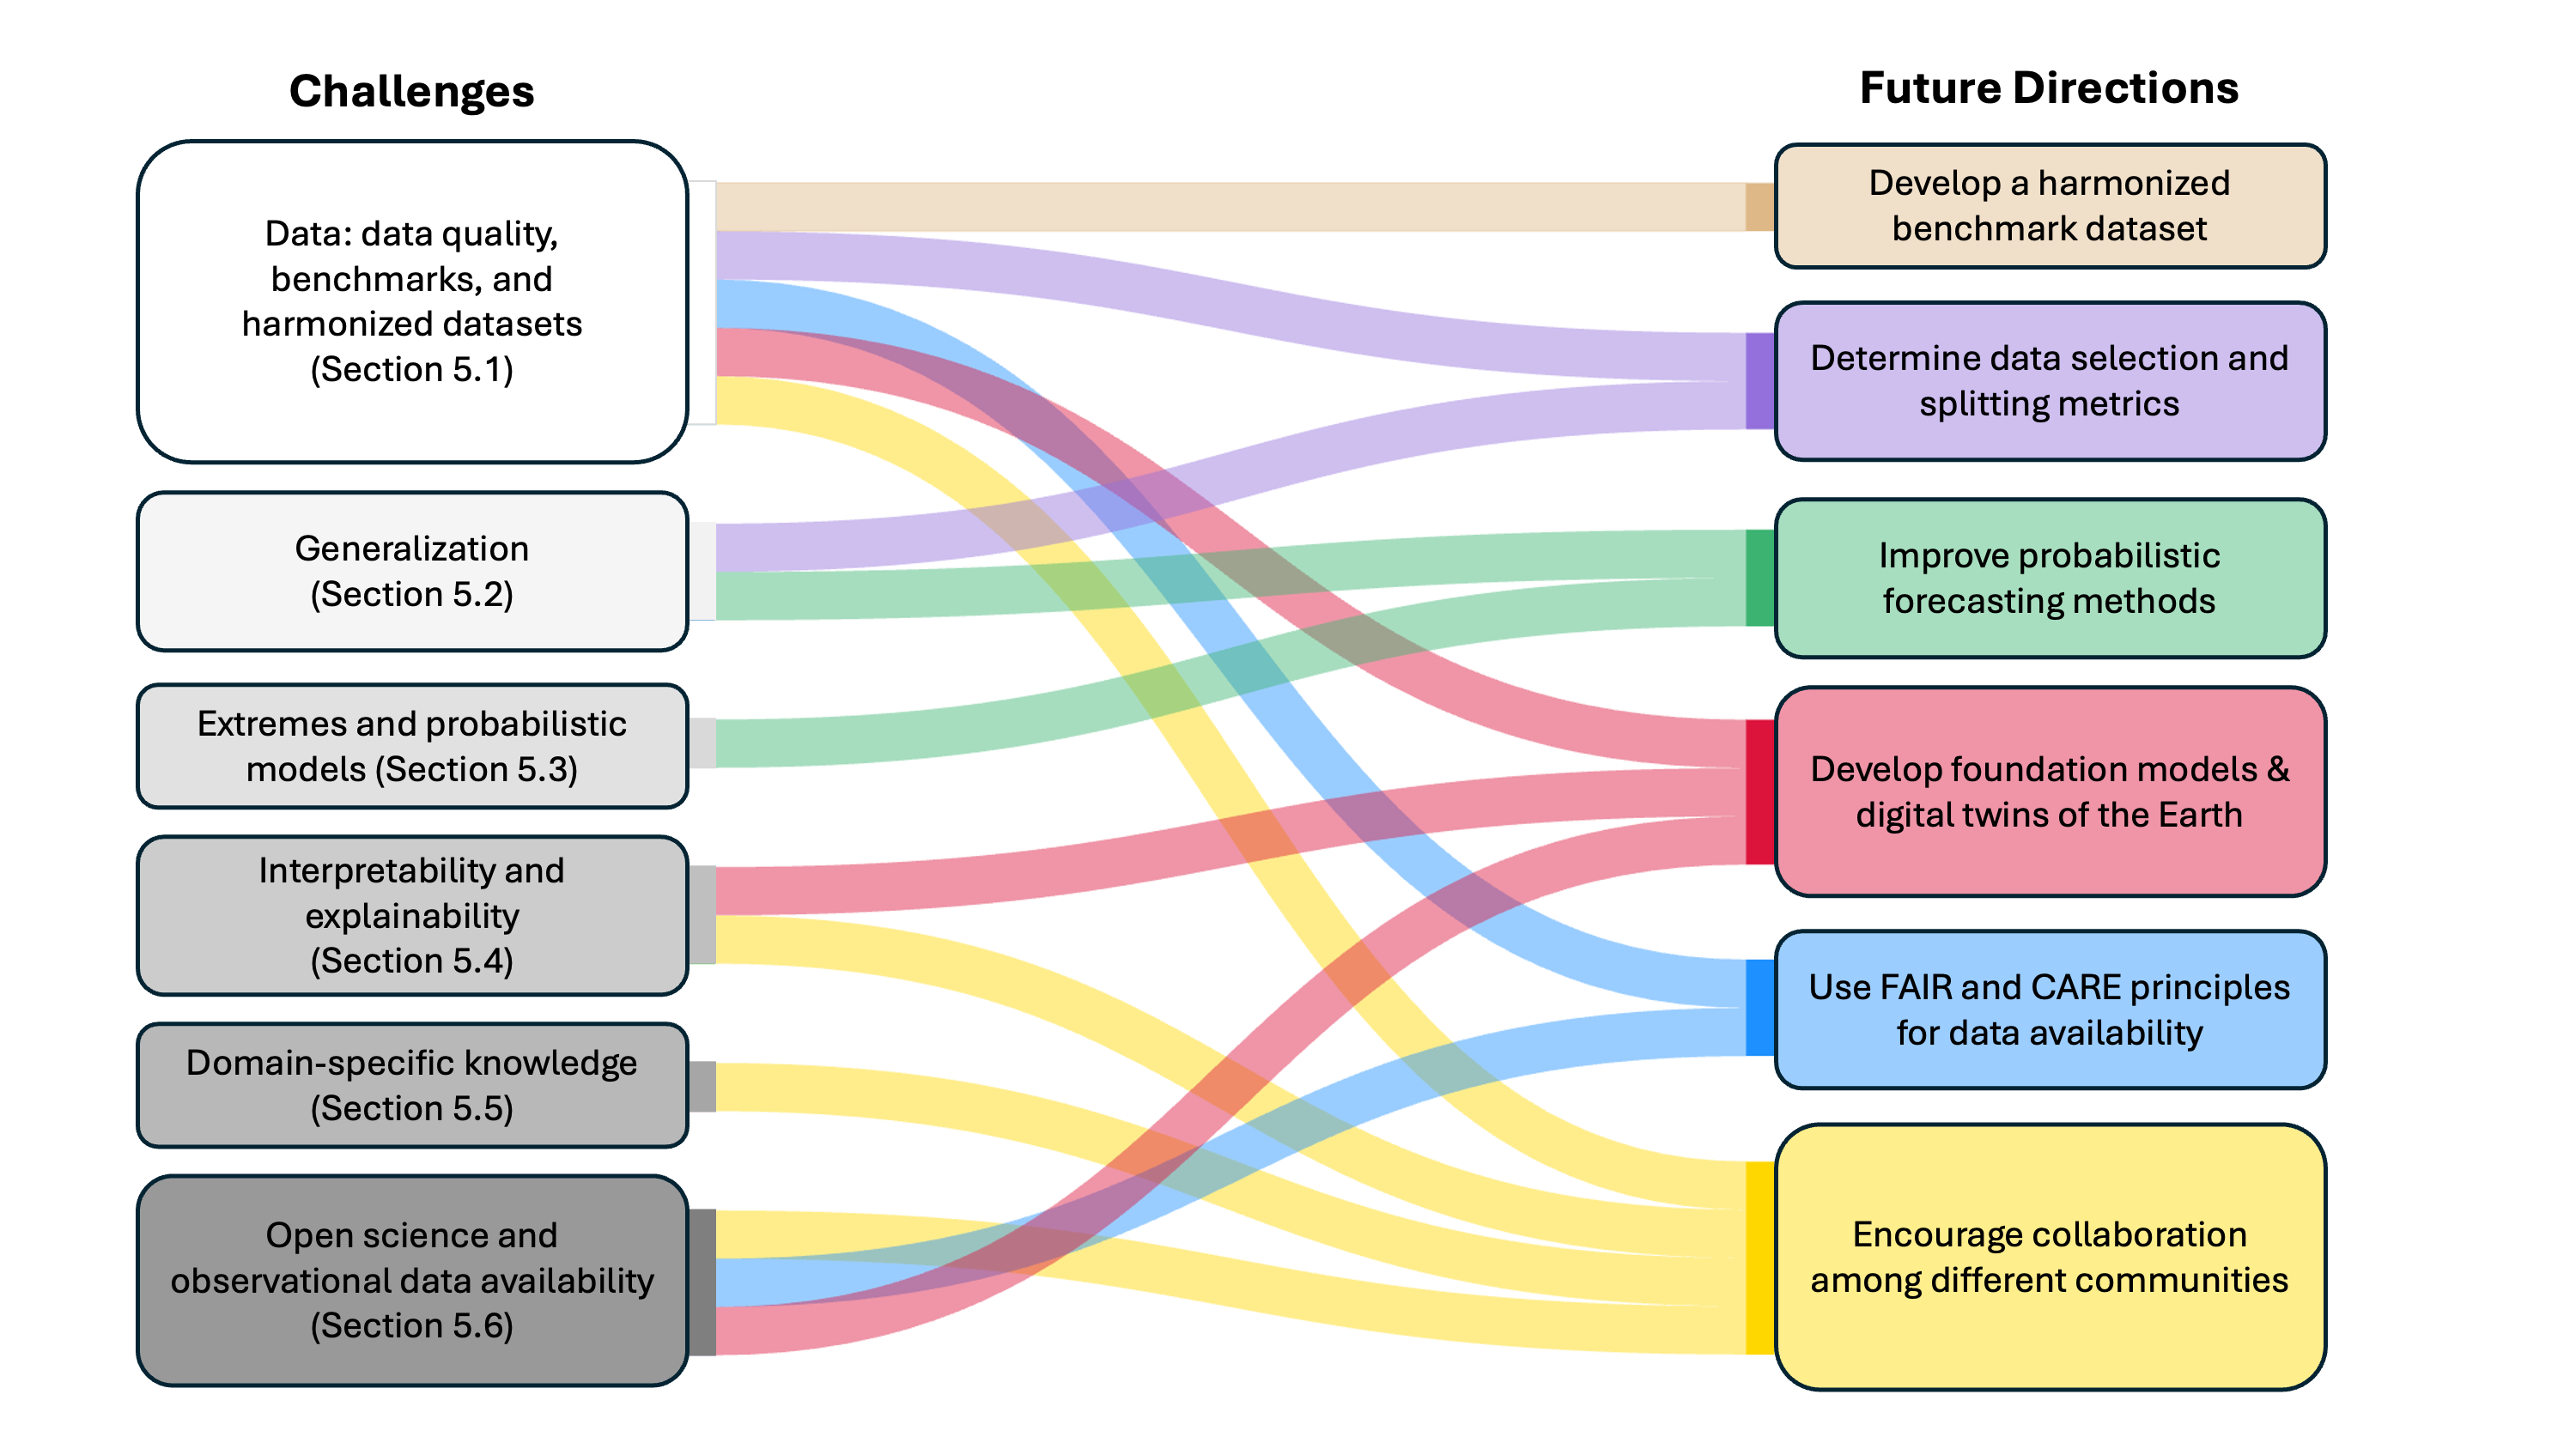
\includegraphics[width=0.85\linewidth]{figures/sankey.png}
    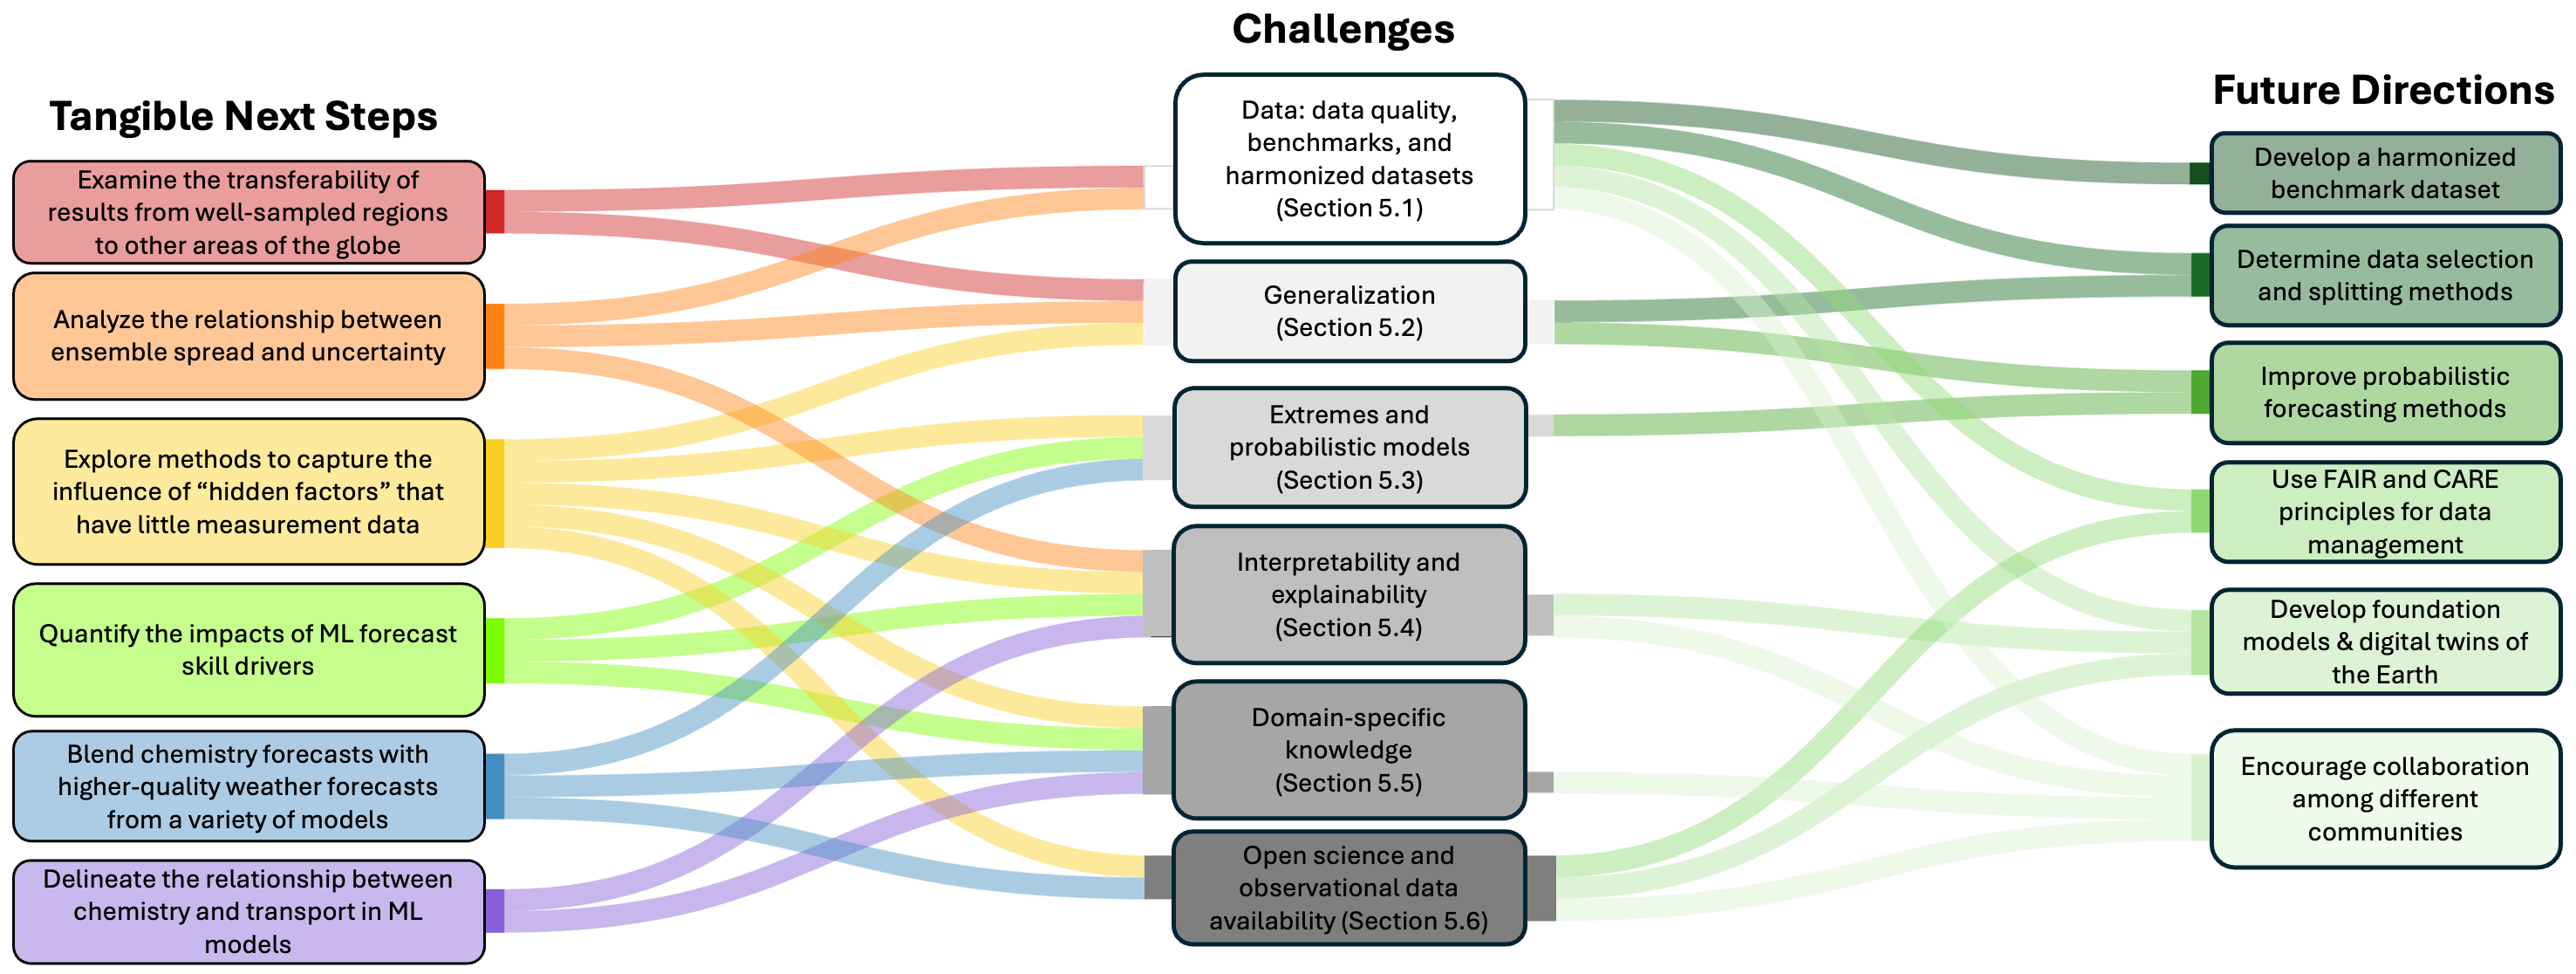
\includegraphics[width=0.99\linewidth]{figures/ML4O3_figure_conclusions_20250626.png}
    \caption{Challenges and future directions described in Sections 5-6. The middle column represents the categories of challenges described in further detail in the sections listed. The left column lists specific projects that could be undertaken to address the challenges. The right column represents general future directions for the ozone AI/ML modeling community to consider. The lines connect categories of challenges with specific future directions and tasks that could address and resolve those challenges.}
    \label{fig:sankey}
\end{figure}

\subsection{The challenges of data availability and workflow }

%As the preceding discussion shows, matching model development to both the available data and the scientific domain is of critical importance.  Indeed, the availability of benchmark datasets is a grand challenge to the field.  

Central to the success of ML modeling efforts and their utility are the choice of datasets and workflows, i.e., ML model choice and training methods. As noted above, in the field of air pollution and atmospheric composition research, the use of ML is hampered by the absence of benchmark datasets suitable for training different model types with varying sizes and complexity. Such well-defined benchmarks including datasets, training objectives, evaluation scores, and baseline models have been instrumental for the rapid development of ML models in other fields  \citep{Dueben2022}. In particular, WeatherBench and WeatherBench2 \citep{Rasp2020, Rasp2024} have been key factors driving the transformation of ML  weather forecasting between 2022 and 2024. A similar dataset to perform the same function for ozone forecasting would allow the robust comparison of different methods, and may guide the field towards more accurate models. Careful curation and data fusion of the TOAR surface ozone database with other relevant datasets might provide a robust and representative benchmark dataset, building on existing work \citep{Betancourt2021}. Ultimately, a lack of sufficient surface observations will impact the study of air quality and downstream impacts on health or vegetation. Therefore improving data coverage over poorly monitored areas remains a priority \citep{Schultz2017}.

%Spatial downscaling of ozone levels using ML approaches may however be an option \citep{Gouldsbrough2024}.
The breadth of information available in datasets like TOAR, GHOST and reanalysis products like Copernicus Atmosphere Monitoring Service (CAMS) is vast, but these products provide significant challenges to the development of ML models for ozone due to heterogeneous data formats and lack of succinct documentation that focuses on the use of such data for ML applications. It may be that ML methods can also be used for infilling missing data (e.g. cloud-filtered satellite data, gaps in in-situ observations) for meteorological variables \citep{Li2023_imputation} and ozone \citep{Arroyo2018, betancourt_global_2022}. Overall, there is a clear need for a harmonized benchmark dataset(s) for ozone to further enable ML models to be developed. These should (as much as possible) follow the vision outlined by \citet{ebert-uphoff_vision_2017} and the principles defined by \citet{Dueben2022}. 

With regards to model choice and development, it is worth noting that, in contrast to CTMs and other methods of simulation, ML models do not \emph{a priori} require simulation, outputting and aggregating of high-resolution time series data to generate predictions for relevant ozone metrics. Instead, ML models can be trained to directly generate forecasts of these metrics (see section~\ref{sec:tsforecast}). In this regard, it is necessary that ozone ML benchmarks should, where appropriate, include target objectives both for forecasting concentrations and for forecasting (a set of) aggregate ozone metrics. See \citet{Fleming2018} and \citet{Lefohn2018} for a more detailed discussion on relevant ozone metrics. 

% choice of model and choice of variables % model training
With regard to ML model training, there is a wide array of data-splitting approaches that can answer subtly related scientific questions. For forecasting it is common practice to divide the data temporally such that the training data completely precedes the testing data, such as using the last few years of a longitudinal dataset for testing. This is commonly recommended in benchmarking studies \citep{lam_learning_2023, Rasp2020}. 
We emphasize that while these procedures likely make intuitive sense, they do not match the default setting in ML packages \citep{schultz_can_2021}, such as scikit-learn \citep{pedregosa_scikit-learn_2011}, where the default cross-validation procedure will randomly split over individual data instances rather than over spatial blocks or temporal blocks. Without using these correct procedures, performance will be overestimated and may not reflect real performance when deployed. In practice, it remains a challenge to carefully define and document the data selection and splitting procedures and adapt them to the scientific problem at hand.

These challenges of data selection and splitting become particularly relevant when looking into climate timescales. Not only can this cause out-of-distribution samples of model input data (for example higher temperatures), but climate change may also affect atmospheric chemical and physical processes so that the mapping between inputs and outputs may drift. This problem is known as 'concept drift', where ML predictions become less accurate over time, which can arise from a non-representative training dataset or an ML model that lacks expressiveness, for example by being unable to extrapolate effectively beyond the bounds of the training data. For the latter, tree-based ML models especially are poor with respect to extremes and outliers. Here, model architecture may play a role. Exploring generative AI models, such as Generative Adversarial Networks (GANs) and transformer models, holds promise for the next generation of ML-based atmospheric models. These newer ML architectures can generate more internally consistent dynamics and require less training data than classical CNNs, while also demonstrating improved accuracy and stability over time. 

%metrics Similar to weather forecasting, there are a range of possible metrics that may characterize a good model of ozone. Unfortunately, the routine use of such metrics for air quality models is not as wide-spread as  the application of essential scores and skill factors in weather forecasting. Essential metrics might include standard deterministic metrics at different forecast lead times, as well as probabilistic metrics such as Continuous Ranked Probability Score (CRPS) for probabilistic models. Metrics targeting extreme event forecast characterisation would be an essential part of this benchmark dataset, which would include a database of observed extreme ozone events. 

\subsection{The challenge of generalization}

In addition to appropriate handling of training data, ensuring the trained model is as generally useful as possible, both in and out of sample, remains an enduring challenge. As is common in ML tasks, models trained on data from one geographical region may not necessarily transfer to another region, even when the underlying task and physics remain the same. This limitation often arises from variations in spurious features or unobserved variables specific to each domain, or differences in emissions and climate in different regions. Many approaches in the ML literature seek to improve the performance of ML models across domains, or under domain shifts, which are yet to be used for ozone forecasting \citep{Sagawa2019}, while recent studies suggest that large-scale weather forecasting models may generalize to unseen conditions and perturbations \citep{Hakim2024}. generalization is particularly important for the use of ML models trained in high-data domains and then deployed in low-data domains. In this context, it may be useful to exploit the benefits of probabilistic forecasting (see following section), using models that report uncertainty in unfamiliar domains.

In the context of observational data, ML is increasingly used to derive or enhance geophysical variables from satellite measurements (see Section 4). However, a conceptual and practical challenge lies in the appropriate application of these ML-derived products across spatio-temporal scales \citep{di_hybrid_2017, zhu_combining_2022, tu_estimation_2023} or atmospheric regimes \citep{ghahremanloo_deep_2023}. There is a need to evaluate and document the scale-dependence of such products, and to guide their use in downstream modeling and analysis applications accordingly.


\subsection{The challenges of extremes and probabilistic models}

A relevant application for ozone forecasting and modeling is the study of extremes, including both accurate forecasting and attribution. Extreme ozone concentrations or fluxes can have a large impact on health and vegetation, and are also referred to as low-likelihood high-impact events. By definition, extreme events occur rarely and are hence challenging to accurately represent. There has been some work on approaches to weight extremes more during model training \citep{Steininger2021}. The ability of models to represent extremes is also an important metric that can be used to evaluate the quality of these models. Extremes can thus play a role for uncertainty quantification of the predictive performance of the models (e.g., important for forecast emulators and assessing ML performance on the extremes), where one can distinguish between epistemic (systematic) and aleatoric (statistical) performance. This connects with an increasingly recognized need to evaluate performance in more rigorous and consistent ways: including the development of new benchmark datasets, diagnostics, and metrics (see above). Progress on ML evaluation include causal evaluation (process-oriented approach) and eXplainable AI (xAI), for understanding (in)consistencies of the ML algorithms with physical processes (in other words: whether accurate answers are found for the right reasons). However, such methods are generally only applicable to relatively small-scale ML models. Dynamical tests and counterfactual experiments provide a means to test the credibility of large ML models \citep{Hakim2024, bano-medina_are_2024}.

Forecasting of potential extreme events is particularly challenging because these events are beyond the typical ozone variability, and naturally, extreme events are rarely and infrequently represented in data. For data-driven models this challenge is further exacerbated by (1) the need to forecast not only the presence of threshold exceedances, but also the intensity and duration of extreme events; and (2) ozone extreme events are often related to other anomalous mechanisms, such as heatwaves and wildfires, which are difficult to take into account based on limited extreme information, also due to the fact that ozone responses to these mechanisms are heterogeneous. Although the extreme value theory is widely adopted, its limitations are frequently acknowledged, including the IID (independent and identically distributed) assumption and independence between extreme and non-extreme events. On the other hand, approaches based on probabilistic forecasting may better characterize the uncertainty and likelihood of extreme events. One solution may be to use metrics and data scenarios to evaluate performance under different types of evaluation scenarios, taking advantage of evaluation metrics in weather forecasting which have been studied extensively. For example, if a key consideration is the ability of a forecasting model to capture extreme events, then metrics that capture relevant performance explicitly on those events should be used. This allows for robust comparison of both the existing and novel models on both traditional metrics and metrics focused on extreme event prediction to more comprehensively evaluate model performance. Evaluation of extreme events is limited in the literature, with recent studies highlighting the lower accuracy of ML models when forecasting spring and summertime ozone concentrations \citep{leufen_o3resnet_2023, Hickman2023}. In addition to helping with forecasting extreme events, probabilistic forecasting more generally provides a number of advantages compared to the deterministic forecasting methods that are currently more common, as outlined in \citet{Bodnar2024}. Furthermore, ML weather forecasting models are increasingly adopting probabilistic and diffusion-based architectures that are able to produce sharp forecasts and uncertainty estimates. This is a promising line of work, however, these ML architectures may be challenging to implement for ozone forecasts due to the %both the dearth of ozone ensemble data (Section 5.1) 
uncertainty driven by the meteorological fields themselves. 

% Well calibrated forecast uncertainty is important for delivering accurate air quality warnings and for public information. Furthermore for other tasks where data quality is critical, such as infilling missing data for use in later analysis, well-calibrated estimates of uncertainty provide information on the quality of ML generated data and hence on further analysis. This is especially relevant as many infilling approaches use average values, and therefore may not be applicable for extremes. 

\subsection{The challenge of interpretability and explainability}
Interpreting and explaining ML models used to study ozone remains difficult. While these two terms are often used interchangeably, for this article we follow the distinction that interpretability focuses on designing and exploring models that are transparent and have comprehensible internal data transformations, whereas explainability methods focus on post-hoc explanations of how black-box models are working \citep{Rudin2019}. Models that are directly and trivially interpretable, such as multiple linear regression, are typically not the most performant, and in the high-data regime, the most performant ML models are typically variants on deep NNs that are difficult to interpret or explain. There is some literature that explores whether PINNs provide more interpretability. For example, efforts are underway to enhance the interpretability of ML models in atmospheric sciences by incorporating or diagnosing conservation priorities such as mass and stoichiometry \citep{sturm_mass-_2020, sturm_conservation_2022}. Additionally, neural operators are being employed to learn the solution operators of ODEs/PDEs from the chemical training data \citep{liu_neural_2024}. However, while incorporating chemistry and physics constraints has been shown to increase interpretability, there is no guarantee that these methods will improve the stability of the ML model over time \citep{sturm_advecting_2023}. Often, there is a trade-off between interpretability and ML model accuracy, especially with more complex models \citep{sengupta_balancing_2023}.
While methods to interpret and explain NNs more generally have been studied widely, mechanistic interpretability of NNs is a challenging task \citep{Nanda2023}, and only a limited range of XAI methods have been tested with ML methods developed for ozone forecasting, often focused on sensitivity approaches which look at the post-hoc explanations where the inputs to models are perturbed to see how predictions change \citep{Ivanovs2021}. Recent studies have investigated the importance of model input parameters through bootstrapping, i.e. random perturbations of individual inputs \citep{Kleinert2021}. Input data perturbation experiments are also possible and informative for very large models as, for example, demonstrated by \citet{Hakim2024} for the Pangu-Weather forecast model. Furthermore, ML approaches are increasingly employed to develop end-to-end models that process raw input data (e.g., emissions, meteorological fields) and directly predict outputs such as ozone concentrations. While end-to-end models bypass the challenges of emulating individual components, which are less prone to short-term instabilities and operator splitting issues, they also limit the ability to track uncertainty metrics tied to physical parameters and processes. 

\subsection{The challenges arising from  domain-specific knowledge}
Modeling ozone using ML proves challenging due to the multitude of sources driving model error (emissions, chemistry, transport, deposition) and the nonlinear response of ozone to these sources. Parameter tuning an appropriate ozone ML model for a complex, high-dimensional parameter space is possible given large computational resources and adaptive learning on pre-defined metrics. However, such an approach is largely inefficient given that atmospheric chemistry data lies on relatively low-dimensional manifolds with respect to the possible input parameter space. That is, many ozone-related relationships are structured with individual signals often being sparse and low-rank. Here, domain knowledge from atmospheric chemistry can help identify the optimal training dataset and define meaningful loss functions and targeted timescales (Figure 1) for the ML model problem. In particular, domain knowledge of chemical and physical processes can help explain errors in ML models at short time scales versus long time scales. For example, ML models of atmospheric chemistry tend to predict well fast chemical processes (e.g., seconds to days) but diverge over longer time scales (e.g., months to years) \citep{kelp_toward_2020}. In addition, knowledge of slow chemical processes, such as the role of peroxyacetyl nitrate (PAN) decomposition for ozone formation over polluted and/or remote areas, may help define appropriate training targets for ML models. An emphasis should be placed on emulating chemistry on longer timescales (>~1 year) as issues of long-range stability are more challenging than shorter-term accuracy, and are a necessity for inclusion into CCMs and ESMs. 

% Indeed, a major long-term goal is the integration of ML-based ozone-related chemistry into physics-based models, such as CCMs and ESMs. While initial efforts have demonstrated promising speedups and reasonable accuracy for short- to medium-term ozone simulations \citep{keller_application_2019, liu_correcting_2022, shen_machine-learning-guided_2022, kelp_online-learned_2022, xia_advancing_2024}, ensuring physical consistency and long-term stability remains a key challenge. In particular, instabilities can arise when neural network components are coupled to stiff chemical schemes or interact with fast transport dynamics, often leading to error growth in remote regions or over extended simulation periods. Future efforts will need to systematically investigate how to mitigate these issues (e.g., through constraint-based learning or regularization techniques), while maintaining computational advantages.

On the other hand, a heightened focus on domain knowledge may unintentionally limit the potential of ML models. Atmospheric chemists typically leverage well-established relationships of the chemical system, such as NO$_X$-limited vs. VOC-limited regimes, which are easily uncovered by linear regression or principal component analysis. By invoking such a strong prior assumption, it may impose constraints that hinder an ML model's ability to learn more complex, non-obvious interactions within the data. This bias toward known relationships risks overlooking patterns that could be hidden in the chemical state space that may promote greater accuracy and stability over longer time scales. Striking a balance between leveraging domain expertise and allowing ML models the flexibility to explore complex dynamics is essential for advancing the predictive capability of ozone modeling.

\subsection{The challenges of open science and observational data availability}

Although an open data infrastructure such as the TOAR-II database gives the impression of low barriers to data access, this might in fact not be true for everyone. Poor internet connectivity from developing countries may limit researchers from retrieving data and subsequently running a computationally demanding model \citep{Blanken2022, Dwivedi2022}. Furthermore, not all possible data providers agree with sending their data to an open access database, which is one important factor that limits global coverage of surface measurement data. The increasing resolution of satellite products and models is often considered to be an improvement, but the larger data size can complicate the processing and analysis of data for some researchers \citep{jain_use_2022}. Some data services require a registration and compliance with data use policies, which could conflict with institutional policies of researchers or exacerbate language barriers that non-native English researchers can experience. Finally, whereas advanced APIs can be ideal for technically skilled researchers and allow for reproducible workflows, they might hinder less technical researchers or policy makers that want to explore data sets.

In particular to developing nations, which may not have the economic ability to acquire high-resolution satellite products outside of those freely-available, it is imperative to develop high-quality, globally generalizable solutions to ozone modeling. Data hosting platforms like Google Earth Engine (GEE) enable users to freely access global data relevant for ozone modeling studies, ranging from land-use information from MODIS \citep{Friedl2021} to human modification data from VIIRS nighttime lights \citep{Elvidge2017}, Gridded Population of the World \citep{CIESIN2018}, and more. Recent work by \citet{Garajeh2023} investigated the ability to detect spatially resolved ozone pollution trends using time-series Sentinel-5 imagery from GEE, highlighting the quality of spatial distribution and accuracy available an open-source product and platform. This demonstrates the necessity to co-design data services and their hosting platforms to provide efficient and performant access to high-quality, well-documented data. 


\section{Future Directions}

% ML is swiftly revolutionizing atmospheric composition research in general, and ozone thermodynamics and chemical processing in particular, harnessing both Earth observations and model outputs to extract insights from vast datasets. 

%%The previous sections have addressed the need for advanced ML techniques, summarized here. Furthermore, we recommend specific, focused projects to address some of the current challenges particular to ozone modeling.

% A wealth of Earth observation data from models, satellites, and in-situ measurements is now available, with data volumes already well beyond tens of petabytes. New developments in deep learning (DL) utilizing this data are rapidly overcoming limitations related to spatiotemporal and multivariate relationships, promising significant breakthroughs \citep{Eyring2024}. However, their direct application to Earth observations is often hindered by challenges such as data quality and coverage, model generalization across different regions, and the complexity of associated metadata.

While new developments have been made in DL to utilize the expansive Earth observation data now available \citep{Eyring2024}, challenges remain regarding the quality, interpretability, and complexity of available data. Also, less work has been done to exploit atmospheric composition datasets, where observations are often less dense and more noisy than weather data. Future research and advancements in observational products suitable for ML, including efforts to address uncertainty quantification \citep[e.g.,][]{Haynes2023}, will enhance our understanding, facilitate process-based model evaluation \citep{Nowack2020}, and enable actionable science. Accurate forecasts of extrema in short-term surface ozone predictions are essential for protecting human health, while reliable projections of long-term changes in tropospheric ozone abundances are critical for understanding climate change and its impacts. Leveraging causal- and physics-constrained data-driven approaches can enhance trust and interpretability in ML-based modeling efforts \citep{Tesch2023,Beucler2024}, and combining causal discovery and xAI methods holds potential for advanced process-based evaluation \citep{IglesiasSuarez2024}. There is a recognized need to evaluate model performance rigorously and consistently, calling for the development of new benchmark datasets, diagnostics, and metrics \citep{Betancourt2021, betancourt_global_2022}, to enable comprehensive evaluation of ML-based ozone modeling techniques. 
% Yet, current domain-specific ML methods and tailored solutions lack a more universal perspective, whereas general-purpose ML-based algorithms may only need to be fine-tuned to address specific tasks. 
To meet society's needs facing current environmental challenges by providing actionable science and maintaining rapid progress in this field, collaboration among atmospheric composition communities and ML communities is essential.

To thrive, the interdisciplinary ozone modeling and forecasting community requires open knowledge sharing, resources and research cooperation. Research in the domain should adhere to the FAIR principles of Findability, Accessibility, Interoperability and Reusability \citep{Wilkinson2008} and the CARE principles of Collective, Authority to control, Responsibility and Ethics \citep{Carroll2021}. Availability of data is essential for data-driven approaches and the developed TOAR-II surface ozone database is essential here through its open data policies and its Application Programming Interface (API), which allow for automatic extraction of data. % Besides the aforementioned “FAIR data”, a call for FAIR-software has been recognized and expressed more recently \citep{Barker2022}, thus including a larger part of the research cycle than only data collection, storage and dissemination.

Future work may focus on foundation models to advance more integrated approaches. These models, trained on extensive datasets in a self-supervised manner \citet{bommasani2021opportunities}, have already demonstrated their capability in fields like weather forecasting and climate science \citep{lessig2023atmorep, nguyen2023climax, Bodnar2024}. In the context of tropospheric ozone modeling, foundation models could improve performance by learning from varied datasets, including observational and numerical modeling data \citep{mukkavilli_ai_2023}. These models are capable of handling multiple air pollutants simultaneously and can incorporate meteorological variables, supporting the development of more comprehensive, flexible and potentially robust air quality benchmarks by harmonizing observational data. Their flexible architectures enable training a single model with large-scale resources and then fine-tuning it for multiple tasks, reducing the computational expense of repeated model training \citep{bommasani2021opportunities}. % For ozone forecasting, they offer a path toward improved modeling capabilities by leveraging diverse data sources and capturing complex relationships in atmospheric composition. 

% Recent work has shown that foundation model architectures can simulate atmospheric dynamics and composition by emulating variables from reanalysis products like CAMS \citep{inness_cams_2019}, achieving promising results for multi-day air pollutants forecasting, including ozone \citep{Bodnar2024}. This shift would, in turn, facilitate the development of models that are not only specific to ozone but capable of generalizing to broader air quality applications, potentially leading to more robust and versatile ML solutions. 

%For CTMs, particularly, and ESMs more broadly, foundation models can serve as valuable tools to either complement or enhance traditional approaches. Chemistry schemes and parameterizations based on ML models can bring computationally efficient interactive chemistry to ESMs for accurate long-term projections \citep{Eyring2016}. Additionally, end-to-end emulators can complement physics-based simulations by employing large ensembles to better constrain uncertainties. While general-purpose ML algorithms, such as foundation models, can provide a step change in data-driven approaches, they may not always lead to actionable science, such as contributing to more informed decision-making by, for example, accurately attributing ozone pollution events to specific sources— and the development of effective mitigation strategies.

At present, there are underexplored opportunities to merge the current successes in ML weather and climate model emulation with CTMs and ESMs. Thus far, atmospheric chemistry data have been largely excluded from ML weather and climate applications, as these current supervised learning frameworks are typically non-extensible, requiring retraining of the entire ML model when incorporating new chemical information. In contrast, unsupervised learning model frameworks, such as pre-trained foundation models, can identify patterns in data without explicit labels, offering a new frontier for ingesting and potentially improving ML modeling of atmospheric chemistry. These foundation models can be fine-tuned on CTM data. For example, the Aurora model \citep{Bodnar2024} is fine-tuned on a subset of six criteria pollutants, including ozone from CAMS \citep{inness_cams_2019}. Fine-tuning ML weather and climate models enables the addition of chemical species to an ML model that is already trained on atmospheric dynamics. This process of fine-tuning, by training specific decoders for new variables, has also recently been carried out for hydrological variables \citep{lehmann2025finetuningweatherfoundationmodel}. However, adding chemical species such as VOCs in the absence of emission inputs (which current models do not consider) on the ML weather model's native 6-hour forecast time steps likely presents challenges. Greater emphasis is needed on understanding the factors influencing ML model performance with respect to the specific challenges of atmospheric composition research and air quality analysis.

%% The need for actionable science to address challenges like climate change and air quality has led to the development of digital twins of the Earth (DTEs), which integrate ML models and physical simulations to provide comprehensive monitoring and forecasting of the Earth system \citep{bauer_digital_2021, Bauer2024}. DTEs enable users to explore “what-if” scenarios by simulating the impacts of various interventions. This user-centric approach contrasts with traditional top-down methods and supports more effective, adaptive responses to environmental challenges. However, the implementation of DTEs raises critical issues regarding governance, data accessibility, and computational demands, particularly as they rely on exascale computing to deliver real-time insights \citep{Hazeleger2024}. As global initiatives like the European Commission’s Destination Earth and NASA’s Earth System Digital Twin advance these frameworks, ML techniques will be essential for ensuring their efficiency and scalability, enabling DTEs to serve as a transformative tool for improving air quality and addressing broader environmental challenges.

% [ADD MARTIN'S TANGIBLE PROJECT SUGGESTIONS HERE] SEE BELOW

While much progress will likely be made by large coordinated efforts to build comprehensive datasets and foundation models (or fine-tune existing foundation models), progress on important problems specific to ozone may be achieved without requiring large-scale, compute-intensive projects (see Figure~\ref{fig:sankey}). First, investigation of the influence of sparsely observed factors on the skill of ozone forecasting models would be useful. For example, VOCs are not widely measured, and the impact of including VOCs as inputs to an ozone forecasting model could be explored. Second, the capacity of models to predict ozone formation in under-observed regions, after being trained on well-sampled regions, may also provide information about the generalizability of ML models. This work could also inform the importance of largely unobserved variables that influence ozone but differ between regions. More generally, a systematic exploration of the factors that influence machine learning model skill in modeling ozone would be useful for the field. In addition, since much data for model training comes from CTMs, which often have degraded resolution compared to the most accurate weather models, improved model accuracy may be obtained by combining high resolution weather models with chemistry data from lower resolution models. This relates to delineating chemistry and transport in models. Since ML models do not explicitly transport chemical tracers, it may be interesting to explore how ML models perform for tracers with different lifetimes. Furthermore, as probabilistic machine learning methods are established for ozone modeling, analyzing the relationship between ensemble spread and ensemble error could be insightful. %in light of the lack of training data, need supersite approach, routine AQ monitoring won't do it. how much and what kind of data are required need to be scoped, e.g. by the approaches above, assess the importance of currently missing variables to ML skill?

\conclusions  %% \conclusions[modified heading if necessary]
While modeling ozone accurately remains a challenging problem across temporal and spatial scales, ML approaches have made progress in a number of areas. As highlighted in this Perspective, ML methods are contributing to research in short-term forecasting, chemistry model emulation, and remote sensing of ozone. Specifically, ML methods are providing increasingly accurate short-term forecasts of ozone at observational stations, and making progress toward providing fast emulators of chemical mechanisms used in chemistry-climate models. In remote sensing, ML methods have shown skill in increasing the efficiency of ozone retrieval, and in making estimates of ozone where there is little satellite coverage. 

Similar to many applications of ML to physical modeling, for our field to make progress in modeling real-world ozone faithfully, models should be trained with a synthesis of high-quality observational datasets and appropriate high-quality benchmarks must be compiled to evaluate the skill of different models, and enable the comparison of ML and numerical models. Furthermore, continued work to mitigate the ozone-specific challenges faced by existing ML models is necessary, as highlighted in Section 6, which will require close collaboration between domain experts and ML researchers to develop models tailored to the particular challenges. Notably for ozone modeling, recent work illustrates that foundation models, trained on diverse datasets, are capable of skillful atmospheric composition modeling. The paradigm of foundation models represents a significant step forward for composition modeling, enabling an integrated approach across multiple scales and tasks, and building on the success of similar models for weather forecasting. Similarly, it remains an open and important question whether ML models can contribute to improved process-level understanding of drivers of ozone, including quantifying the influence of sparsely observed drivers, and generalize to unseen air pollution and climate scenarios.

As ML continues to transform ozone research and adjacent fields, including weather and climate modeling, the ozone modeling community needs to ensure future research builds on strong foundations. By developing robust benchmarks, building productive cross-disciplinary collaborations, and embracing state-of-the-art techniques, ML-driven ozone research has the potential to not only advance scientific understanding but also deliver actionable benefits for climate resilience and public health.



%% The following commands are for the statements about the availability of data sets and/or software code corresponding to the manuscript.
%% It is strongly recommended to make use of these sections in case data sets and/or software code have been part of your research the article is based on.

%\codeavailability{TEXT} %% use this section when having only software code available


%\dataavailability{TEXT} %% use this section when having only data sets available


\appendix
\section{Glossary}    %% Appendix A



\title{Glossary of terms and abbreviations}

\begin{description}[style=nextline]

\item[Artificial Intelligence (AI):] A software or model that is capable of performing tasks that typically require human intelligence.

\item[Copernicus Atmosphere Monitoring Service (CAMS):] A service by the EU Earth observation programme to provide comprehensive data on atmospheric composition and air quality through satellite and ground-based monitoring.

\item[Chemistry-Climate Model (CCM):] A type of global model focused on the interactions between atmospheric chemistry and climate.

\item[Convolutional Neural Network (CNN):] A type of neural network designed for processing data with grid structure, often used for image processing.

\item[Chemical Transport Model (CTM):] A type of global model designed to simulate the movement and chemical reactions of atmospheric pollutants.

\item[Deep Forest (DF):] A deep learning architecture based on decision trees instead of neural networks.

\item[Deep Learning (DL):] A field of machine learning focused on the development and use of neural networks.

\item[Decision Tree (DT):] A hierarchical supervised learning algorithm, often used to create classification and regression models.

\item[Earth System Model (ESM):] A global model that simulates all aspects of the Earth system, including the interactions between the atmosphere, oceans, land, and biosphere.

\item[Feed-forward Neural Network (FNN):] A basic type of neural network where data move in one direction without feedback loops, often used for data classification and recognition.

\item[Foundation Model (FM):] A machine learning model trained on vast amounts of data, designed to be adapted to a broad range of tasks.

\item[Generative Adversarial Network (GAN):] A type of machine learning technique where two neural networks compete unsupervised to produce the most accurate result.

\item[General Circulation Model (GCM):] A global model that simulates the Earth’s atmospheric dynamics and circulation.

\item[Gradient Boosted Decision Tree (GBDT):] An ensemble machine learning technique that uses the results of multiple decision trees to improve accuracy and reduce error of the prediction.

\item[Large Language Model (LLM):] A type of foundation model trained on very large text datasets to understand and generate natural language.

\item[Long Short-Term Memory network (LSTM):] A type of recurrent neural network designed to retain information over longer sequences for longer periods.

\item[Machine Learning (ML):] A field of artificial intelligence dedicated to algorithms and models that can learn and make predictions from the input data without being explicitly programmed to do so.

\item[Neural Network (NN):] A machine learning model designed to process data in a similar way as the human brain.

\item[Physics-Informed Neural Network (PINN):] A type of neural network trained to follow known physical laws.

\item[Random Forest (RF):] An ensemble machine learning algorithm that combines multiple decision trees during the training process to improve prediction accuracy and reduce overfitting.

\item[Recurrent Neural Networks (RNN):] A type of neural network in which data can loop back into the network retaining memory of previous inputs. It is designed for sequential data processing where context is important, such as natural language and time series.

\item[Transformer Model (TM):] A type of deep learning model that converts a given input into a desired output, learning context and meaning. It is used as a foundation model for large language models as an alternative to CNNs and RNNs architectures.

\item[U-Net:] A type of convolutional neural network designed for image segmentation and de-noising.

\item[eXplainable AI (xAI):] A type of artificial intelligence that provides the information necessary to understand how a certain output was achieved.

\end{description}


\codedataavailability{All code and plotting routines are available at \citep  {ML4O3_repository}.} %% use this section when having data sets and software code available

%\newpage

\authorcontribution{All  authors contributed to the writing and review of the manuscript.  SHMH, MK, PTG, F-IS, GK, KD, KZ, MGS and EAP  led the writing and preparation of the MS.  SHMH led Section 2,  MK  section 3, KD, EAP and KM led section 4, GK section 5 and FI-S section 6.  } %% this section is mandatory

\competinginterests{S.H.M.H., M.K., D.E.C., P.T.G. declare no competing interests. Some of the authors are involved with editorial work for Copernicus journals.} %% this section is mandatory even if you declare that no competing interests are present

%\disclaimer{TEXT} %% optional section

\begin{acknowledgements}
S.H.M.H. acknowledges funding from EPSRC via the AI4ER CDT at the University of Cambridge (EP/S022961/1). P.T.G. acknowledges the Environmental Geochemical Cycle Research Group, Earth Surface System Research Center, Japan Agency For Marine Science and Technology for support as an External Researcher, and the Global Atmospheric Chemistry Section, Earth System Division,  National Institute for Environmental Studies, Tsukuba, Japan for support as a visiting scientist in 2024. P.T.G. and A.T.A. were financially supported by NERC through NCAS (R8/H12/83/003).  Part of this work was conducted at the Jet Propulsion Laboratory, California Institute of Technology, under contract with the NASA. We acknowledge the support of the National Aeronautics and Space Administration (NASA) Atmospheric Composition: Aura Science Team Program (19-AURAST19-0044), Atmospheric Composition Modeling and Analysis Program (22-ACMAP22-0013), NASA Earth Science U.S. Participating Investigator program (22-EUSPI22-0005).
Z.L. was acknowledges the National Natural Science Foundation of China,  grant number 42307140. MGS acknowledges funding by the European Commission under grant ERC-AdvG-787576.  K.-L.C. was supported by NOAA cooperative agreement (no. NA22OAR4320151).  J.J.W. acknowledges National Aeronautics and Space Administration (NASA) grants no. NNX16AQ30G and no. 80NSSC23K0930.  D.E.C. acknowledges financial support from Underwriters Laboratories, Inc.


\end{acknowledgements}


%% REFERENCES

%% The reference list is compiled as follows:

%% Since the Copernicus LaTeX package includes the BibTeX style file copernicus.bst,
%% authors experienced with BibTeX only have to include the following two lines:
%%
%% \bibliographystyle{copernicus}
%% \bibliography{example.bib}
%%
%% URLs and DOIs can be entered in your BibTeX file as:
%%
%% URL = {http://www.xyz.org/~jones/idx_g.htm}
%% DOI = {10.5194/xyz}
\bibliographystyle{copernicus}
\bibliography{references_ML4O3}
%\subsection{}     %% Appendix A1, A2, etc.


\noappendix       %% use this to mark the end of the appendix section. Otherwise the figures might be numbered incorrectly (e.g. 10 instead of 1).

%% Regarding figures and tables in appendices, the following two options are possible depending on your general handling of figures and tables in the manuscript environment:

%% Option 1: If you sorted all figures and tables into the sections of the text, please also sort the appendix figures and appendix tables into the respective appendix sections.
%% They will be correctly named automatically.

%% Option 2: If you put all figures after the reference list, please insert appendix tables and figures after the normal tables and figures.
%% To rename them correctly to A1, A2, etc., please add the following commands in front of them:

\appendixfigures  %% needs to be added in front of appendix figures

\appendixtables   %% needs to be added in front of appendix tables

%% Please add \clearpage between each table and/or figure. Further guidelines on figures and tables can be found below.





%% FIGURES

%% When figures and tables are placed at the end of the MS (article in one-column style), please add \clearpage
%% between bibliography and first table and/or figure as well as between each table and/or figure.

% The figure files should be labelled correctly with Arabic numerals (e.g. fig01.jpg, fig02.png).


%% ONE-COLUMN FIGURES

%%f
%\begin{figure}[t]
%\includegraphics[width=8.3cm]{FILE NAME}
%\caption{TEXT}
%\end{figure}
%
%%% TWO-COLUMN FIGURES
%
%%f
%\begin{figure*}[t]
%\includegraphics[width=12cm]{FILE NAME}
%\caption{TEXT}
%\end{figure*}
%
%
%%% TABLES
%%%
%%% The different columns must be seperated with a & command and should
%%% end with \\ to identify the column brake.
%
%%% ONE-COLUMN TABLE
%
%%t
%\begin{table}[t]
%\caption{TEXT}
%\begin{tabular}{column = lcr}
%\tophline
%
%\middlehline
%
%\bottomhline
%\end{tabular}
%\belowtable{} % Table Footnotes
%\end{table}
%
%%% TWO-COLUMN TABLE
%
%%t
%\begin{table*}[t]
%\caption{TEXT}
%\begin{tabular}{column = lcr}
%\tophline
%
%\middlehline
%
%\bottomhline
%\end{tabular}
%\belowtable{} % Table Footnotes
%\end{table*}
%
%%% LANDSCAPE TABLE
%
%%t
%\begin{sidewaystable*}[t]
%\caption{TEXT}
%\begin{tabular}{column = lcr}
%\tophline
%
%\middlehline
%
%\bottomhline
%\end{tabular}
%\belowtable{} % Table Footnotes
%\end{sidewaystable*}
%


\end{document}
